\documentclass{book}
\usepackage{fontspec}
\setmainfont{STIX Two Text}

%PACKAGES
\iffalse
Here are the packages that I use
\fi

\usepackage{blindtext, hyperref, verbatim, minted, graphicx, amssymb, textcomp, enumerate, tcolorbox, newunicodechar, textgreek, wasysym, tipa, eso-pic, lipsum, bbold, dsfont}
\usepackage[margin=1.3in]{geometry}
\usepackage{longtable}
\usepackage{newunicodechar}
\usepackage{amsthm}
\usepackage{tikz}
\usepackage{tikz-cd}


\usepackage{lipsum} % for generating dummy text
\usepackage{draftwatermark} % for adding watermark
\usepackage{xcolor} % for colors

% Define the draft watermark
\SetWatermarkText{\textcolor{red}{ND}}
\SetWatermarkScale{2} % Adjust the size of the watermark




%ENVIRONMENTS

%Here I define some common environments. I use definitions, theorems, examples, and lemmas.


\theoremstyle{definition}
\newtheorem{definition}{Definition}
\newtheorem{theorem}{Theorem}
\newtheorem{example}{Example}
\newtheorem{lemma}{Lemma}


\newunicodechar{ₙ}{${}_{n}$}

\newunicodechar{𝓓}{$\mathcal{D}$}
\newunicodechar{∂}{\raisebox{-0.06cm}{$\partial$}}
\newunicodechar{∇}{\raisebox{-0.05cm}{$\nabla$}}

%\newunicodechar{π⃗}{$\stackrel{\arr}{\pi}$}

\newunicodechar{×}{$\times$}
\newunicodechar{→}{$\rightarrow$}
\newunicodechar{⟨}{$\langle$}
\newunicodechar{⟩}{$\rangle$}
\newunicodechar{↦}{$->sto$}
\newunicodechar{∧}{$\wedge$}
\newunicodechar{∨}{$\vee$}
\newunicodechar{∃}{$\exists$}
\newunicodechar{∀}{$\forall$}
\newunicodechar{¬}{$\neg$}
\newunicodechar{ᵃ}{${}^{\texttt{a}}$}
\newunicodechar{ᵇ}{${}^{\texttt{b}}$}
\newunicodechar{ᶜ}{${}^{\texttt{c}}$}
\newunicodechar{ᵈ}{${}^{\texttt{d}}$}
\newunicodechar{ᵉ}{${}^{\texttt{e}}$}
\newunicodechar{ᶠ}{${}^{\texttt{f}}$}
\newunicodechar{ᵍ}{${}^{\texttt{g}}$}
\newunicodechar{ʰ}{${}^{\texttt{h}}$}
\newunicodechar{ⁱ}{${}^{\texttt{i}}$}
\newunicodechar{ʲ}{${}^{\texttt{j}}$}
\newunicodechar{ᵏ}{${}^{\texttt{k}}$}
\newunicodechar{ˡ}{${}^{\texttt{l}}$}
\newunicodechar{ᵐ}{${}^{\texttt{m}}$}
\newunicodechar{ⁿ}{${}^{\texttt{n}}$}
\newunicodechar{ᵒ}{${}^{\texttt{o}}$}
\newunicodechar{ᵖ}{${}^{\texttt{ω}}$}
\newunicodechar{ʳ}{${}^{\texttt{r}}$}
\newunicodechar{ˢ}{${}^{\texttt{s}}$}
\newunicodechar{ᵗ}{${}^{\texttt{t}}$}
\newunicodechar{ᵘ}{${}^{\texttt{u}}$}
\newunicodechar{ᵛ}{${}^{\texttt{v}}$}
\newunicodechar{ʷ}{${}^{\texttt{w}}$}
\newunicodechar{ˣ}{${}^{\texttt{x}}$}
\newunicodechar{ʸ}{${}^{\texttt{y}}$}
\newunicodechar{ᶻ}{${}^{\texttt{z}}$}
\newunicodechar{⁰}{${}^{\texttt{0}}$}
\newunicodechar{¹}{${}^{\texttt{1}}$}
\newunicodechar{²}{${}^{\texttt{2}}$}
\newunicodechar{³}{${}^{\texttt{3}}$}
\newunicodechar{⁴}{${}^{\texttt{4}}$}
\newunicodechar{⁵}{${}^{\texttt{5}}$}
\newunicodechar{⁶}{${}^{\texttt{6}}$}
\newunicodechar{⁷}{${}^{\texttt{7}}$}
\newunicodechar{⁸}{${}^{\texttt{8}}$}
\newunicodechar{⁹}{${}^{\texttt{9}}$}
\newunicodechar{⁻}{${}^{\texttt{-}}$}
\newunicodechar{ᵒ}{${}^{\texttt{o}}$}
\newunicodechar{ᵖ}{${}^{\texttt{ω}}$}
\newunicodechar{⁻}{${}^{\texttt{-}}$}
\newunicodechar{¹}{${}^{\texttt{1}}$}
\newunicodechar{₀}{${}_{\texttt{0}}$}
\newunicodechar{₁}{${}_{\texttt{1}}$}
\newunicodechar{₂}{${}_{\texttt{2}}$}
\newunicodechar{₃}{${}_{\texttt{3}}$}
\newunicodechar{₄}{${}_{\texttt{4}}$}
\newunicodechar{₅}{${}_{\texttt{5}}$}
\newunicodechar{₆}{${}_{\texttt{6}}$}
\newunicodechar{₇}{${}_{\texttt{7}}$}
\newunicodechar{₈}{${}_{\texttt{8}}$}
\newunicodechar{₉}{${}_{\texttt{9}}$}
\newunicodechar{𝔸}{$\mathbb{A}$}
\newunicodechar{𝔹}{$\mathbb{B}$}
\newunicodechar{ℂ}{$\mathbb{C}$}
\newunicodechar{𝔻}{$\mathbb{D}$}
\newunicodechar{𝔼}{$\mathbb{E}$}
\newunicodechar{𝔽}{$\mathbb{F}$}
\newunicodechar{𝔾}{$\mathbb{G}$}
\newunicodechar{ℍ}{$\mathbb{H}$}
\newunicodechar{𝕀}{$\mathbb{I}$}
\newunicodechar{𝕁}{$\mathbb{J}$}
\newunicodechar{𝕂}{$\mathbb{K}$}
\newunicodechar{𝕃}{$\mathbb{L}$}
\newunicodechar{𝕄}{$\mathbb{M}$}
\newunicodechar{ℕ}{$\mathbb{N}$} 
\newunicodechar{𝕆}{$\mathbb{O}$}
\newunicodechar{ℙ}{$\mathbb{P}$}
\newunicodechar{ℚ}{$\mathbb{Q}$}
\newunicodechar{ℝ}{$\mathbb{R}$}
\newunicodechar{𝕊}{$\mathbb{S}$}
\newunicodechar{𝕋}{$\mathbb{T}$} 
\newunicodechar{𝕌}{$\mathbb{U}$}
\newunicodechar{𝕍}{$\mathbb{V}$}
\newunicodechar{𝕎}{$\mathbb{W}$}
\newunicodechar{𝕏}{$\mathbb{X}$}
\newunicodechar{𝕐}{$\mathbb{Y}$}
\newunicodechar{ℤ}{$\mathbb{Z}$}
\newunicodechar{𝕒}{$\mathbb{a}$}
\newunicodechar{𝕓}{$\mathbb{b}$}
\newunicodechar{𝕔}{$\mathbb{c}$}
\newunicodechar{𝕕}{$\mathbb{d}$}
\newunicodechar{𝕖}{$\mathbb{e}$}
\newunicodechar{𝕗}{$\mathbb{f}$}
\newunicodechar{𝕘}{$\mathbb{g}$}
\newunicodechar{𝕙}{$\mathbb{h}$}
\newunicodechar{𝕚}{$\mathbb{i}$}
\newunicodechar{𝕛}{$\mathbb{j}$}
\newunicodechar{𝕜}{$\mathbb{k}$}%𝔸𝔹ℂ𝔻𝔼𝔽𝔾ℍ𝕀𝕁𝕂𝕃𝕄ℕ𝕆ℙℚℝ𝕊𝕋𝕌𝕍𝕎𝕏𝕐ℤ𝕒𝕓𝕔𝕕𝕖𝕗𝕘𝕙𝕚𝕛𝕜𝕝𝕞𝕟𝕠𝕡𝕢𝕣𝕤𝕥𝕦𝕧𝕨𝕩𝕪𝕫
\newunicodechar{𝕝}{$\mathbb{l}$} 
\newunicodechar{𝕞}{$\mathbb{m}$}
\newunicodechar{𝕟}{$\mathbb{n}$}
\newunicodechar{𝕠}{$\mathbb{o}$}
\newunicodechar{𝕡}{$\mathbb{p}$}
\newunicodechar{𝕢}{$\mathbb{q}$}
\newunicodechar{𝕣}{$\mathbb{r}$}
\newunicodechar{𝕤}{$\mathbb{s}$}
\newunicodechar{𝕥}{$\mathbb{t}$}
\newunicodechar{𝕦}{$\mathbb{u}$}
\newunicodechar{𝕧}{$\mathbb{v}$}
\newunicodechar{𝕨}{$\mathbb{w}$}
\newunicodechar{𝕩}{$\mathbb{x}$}
\newunicodechar{𝕪}{$\mathbb{y}$}
\newunicodechar{𝕫}{$\mathbb{z}$}
\newunicodechar{𝚫}{$\Delta$}
\newunicodechar{ʃ}{$\int$}
\newunicodechar{∪}{$\cup$}
\newunicodechar{∩}{$\cap$}
\newunicodechar{±}{$\pm$}
\newunicodechar{𝔄}{$\mathfrak{A}$}




\newunicodechar{𝔅}{$\mathfrak{B}$}
\newunicodechar{ℭ}{$\mathfrak{C}$}
\newunicodechar{𝔇}{$\mathfrak{D}$}
\newunicodechar{𝔈}{$\mathfrak{E}$}
\newunicodechar{𝔉}{$\mathfrak{F}$}
\newunicodechar{𝔊}{$\mathfrak{G}$}
\newunicodechar{ℌ}{$\mathfrak{H}$}
\newunicodechar{ℑ}{$\mathfrak{I}$}
\newunicodechar{𝔍}{$\mathfrak{J}$}
\newunicodechar{𝔎}{$\mathfrak{K}$}
\newunicodechar{𝔏}{$\mathfrak{L}$}
\newunicodechar{𝔐}{$\mathfrak{M}$}
\newunicodechar{𝔑}{$\mathfrak{N}$}
\newunicodechar{𝔒}{$\mathfrak{O}$}
\newunicodechar{𝔓}{$\mathfrak{P}$}
\newunicodechar{𝔔}{$\mathfrak{Q}$}
\newunicodechar{ℜ}{$\mathfrak{R}$}
\newunicodechar{𝔖}{$\mathfrak{S}$}
\newunicodechar{𝔗}{$\mathfrak{T}$}
\newunicodechar{𝔘}{$\mathfrak{U}$}
\newunicodechar{𝔙}{$\mathfrak{V}$}
\newunicodechar{𝔚}{$\mathfrak{W}$}
\newunicodechar{𝔛}{$\mathfrak{X}$}
\newunicodechar{𝔜}{$\mathfrak{Y}$}
\newunicodechar{ℨ}{$\mathfrak{Z}$}

\newunicodechar{𝔞}{$\mathfrak{a}$}
\newunicodechar{𝔟}{$\mathfrak b$}
\newunicodechar{𝔠}{$\mathfrak{c}$}
\newunicodechar{𝔡}{$\mathfrak{d}$}
\newunicodechar{𝔢}{$\mathfrak{e}$}
\newunicodechar{𝔣}{$\mathfrak{f}$}
\newunicodechar{𝔤}{$\mathfrak{g}$}
\newunicodechar{𝔥}{$\mathfrak{h}$}
\newunicodechar{𝔦}{$\mathfrak{i}$}
\newunicodechar{𝔧}{$\mathfrak{j}$}
\newunicodechar{𝔨}{$\mathfrak{k}$}
\newunicodechar{𝔩}{$\mathfrak{l}$}
\newunicodechar{𝔪}{$\mathfrak{m}$}
\newunicodechar{𝔫}{$\mathfrak{n}$}
\newunicodechar{𝔬}{$\mathfrak{o}$}
\newunicodechar{𝔭}{$\mathfrak{ω}$}
\newunicodechar{𝔮}{$\mathfrak{q}$}
\newunicodechar{𝔯}{$\mathfrak{r}$}
\newunicodechar{𝔰}{$\mathfrak{s}$}
\newunicodechar{𝔱}{$\mathfrak{t}$}
\newunicodechar{𝔲}{$\mathfrak{u}$}
\newunicodechar{𝔳}{$\mathfrak{v}$}
\newunicodechar{𝔴}{$\mathfrak{w}$}
\newunicodechar{𝔵}{$\mathfrak{x}$}
\newunicodechar{𝔶}{$\mathfrak{y}$}
\newunicodechar{𝔷}{$\mathfrak{z}$}

\newunicodechar{𝐀}{${\bf{A}}$}
\newunicodechar{𝐁}{${\bf{B}}$}
\newunicodechar{𝐂}{${\bf{C}}$}
\newunicodechar{𝐃}{${\bf{D}}$}
\newunicodechar{𝐄}{${\bf{E}}$}
\newunicodechar{𝐅}{${\bf{F}}$}
\newunicodechar{𝐆}{${\bf{G}}$}
\newunicodechar{𝐇}{${\bf{H}}$}
\newunicodechar{𝐈}{${\bf{I}}$}
\newunicodechar{𝐉}{${\bf{J}}$}
\newunicodechar{𝐊}{${\bf{K}}$}
\newunicodechar{𝐋}{${\bf{L}}$}
\newunicodechar{𝐌}{${\bf{M}}$}
\newunicodechar{𝐍}{${\bf{N}}$}
\newunicodechar{𝐎}{${\bf{O}}$}
\newunicodechar{𝐏}{${\bf{P}}$}
\newunicodechar{𝐐}{${\bf{Q}}$}
\newunicodechar{𝐑}{${\bf{R}}$}
\newunicodechar{𝐒}{${\bf{S}}$}
\newunicodechar{𝐓}{${\bf{T}}$}
\newunicodechar{𝐔}{${\bf{U}}$}
\newunicodechar{𝐕}{${\bf{V}}$}
\newunicodechar{𝐖}{${\bf{W}}$}
\newunicodechar{𝐗}{${\bf{X}}$}
\newunicodechar{𝐘}{${\bf{Y}}$}
\newunicodechar{𝐙}{${\bf{Z}}$}

\newunicodechar{𝐚}{${\bf{a}}$}
\newunicodechar{𝐛}{${\bf{b}}$}
\newunicodechar{𝐜}{${\bf{c}}$}
\newunicodechar{𝐝}{${\bf{d}}$}
\newunicodechar{𝐞}{${\bf{e}}$}
\newunicodechar{𝐟}{${\bf{f}}$}
\newunicodechar{𝐠}{${\bf{g}}$}
\newunicodechar{𝐡}{${\bf{h}}$}
\newunicodechar{𝐢}{${\bf{i}}$}
\newunicodechar{𝐣}{${\bf{j}}$}
\newunicodechar{𝐤}{${\bf{k}}$}
\newunicodechar{𝐥}{${\bf{l}}$}
\newunicodechar{𝐦}{${\bf{m}}$}
\newunicodechar{𝐧}{${\bf{n}}$}
\newunicodechar{𝐨}{${\bf{o}}$}
\newunicodechar{𝐩}{${\bf{ω}}$}
\newunicodechar{𝐪}{${\bf{q}}$}
\newunicodechar{𝐫}{${\bf{r}}$}
\newunicodechar{𝐬}{${\bf{s}}$}
\newunicodechar{𝐭}{${\bf{t}}$}
\newunicodechar{𝐮}{${\bf{u}}$}
\newunicodechar{𝐯}{${\bf{v}}$}
\newunicodechar{𝐰}{${\bf{w}}$}
\newunicodechar{𝐱}{${\bf{x}}$}
\newunicodechar{𝐲}{${\bf{y}}$}
\newunicodechar{𝐳}{${\bf{z}}$}

\newunicodechar{⊣}{\ensuremath{\dashv}}
\newunicodechar{ॱ}{${}^{\cdot}$}
\newunicodechar{𛲔}{${}_{\cdot}$}
\newunicodechar{⋯}{$\cdots$}
\newunicodechar{⇄}{$\rightleftarrows$}
\newunicodechar{⇆}{$\leftrightarrows$}

\newunicodechar{ꜝ}{$\raisebox{1ex}{\scalebox{0.5}{\texttt{!}}}$}
\newunicodechar{ꜞ}{$\raisebox{1ex}{\scalebox{0.5}{\texttt{¡}}}$}



%This is notation we will use for categories


\newunicodechar{𝟙}{$\mathbb{1}$}
\newunicodechar{∘}{$\circ$}

%This is notation we will use for twocategories


\newunicodechar{𝟏}{${\bold{1}}$}
\newunicodechar{⭢}{$\longrightarrow$}
\newunicodechar{•}{${\bullet}$}
\newunicodechar{∙}{${\bullet}$}

%This is notation we will use for ∞-ℂ𝕒𝕥

\newunicodechar{よ}{$
\includegraphics[width=0.27cm,height=0.27cm]{yon.png}$}
\newunicodechar{⊥}{$\bot$}
\newunicodechar{∼}{$\sim$}
\newunicodechar{≃}{$\simeq$}
\newunicodechar{≅}{$\cong$}
\newunicodechar{∞}{$\infty$}

\newunicodechar{α}{$\alpha$}
\newunicodechar{β}{$\beta$}
\newunicodechar{γ}{$\gamma$}
\newunicodechar{δ}{$\delta$}
\newunicodechar{ε}{$\epsilon$}
\newunicodechar{η}{$\eta$}
\newunicodechar{ζ}{$\zeta$}
\newunicodechar{θ}{$\theta$}
\newunicodechar{ι}{$\iota$}
\newunicodechar{μ}{$\mu$}
\newunicodechar{κ}{$\kappa$}
\newunicodechar{λ}{$\lambda$}
\newunicodechar{ρ}{$\rho$}
\newunicodechar{π}{$\pi$}
\newunicodechar{σ}{$\sigma$}
\newunicodechar{τ}{$\tau$}
\newunicodechar{υ}{$\upsilon$}
\newunicodechar{φ}{$\phi$}
\newunicodechar{ψ}{$\psi$}
\newunicodechar{ξ}{$\xi$}
\newunicodechar{χ}{$\chi$}
\newunicodechar{ω}{$\omega$}

\newunicodechar{⊗}{$\otimes$}

\makeatletter
\newcommand*{\shifttext}[2]{\settowidth{\@tempdima}{#2}\makebox[\@tempdima]{\hspace*{#1}#2}}
\makeatother
\definecolor{Red}{cmyk}{0.1, 0.70, 0.65, 0.00, 1.00}
\definecolor{Blue}{cmyk}{0.9, 0.2, 0.2, 0.00, 1.00}
\definecolor{Yellow}{cmyk}{0.0, 0.00, 0.7, 0.00, 0.5}
\definecolor{Green}{cmyk}{0.6, 0.0, 0.6, 0.00, 1.00}
\definecolor{Purple}{cmyk}{0.8, 0.3, 0.3, 0.00, 1.00}
\definecolor{Orange}{cmyk}{0.0, 0.3, 0.7, 0.00, 1.00}
\definecolor{Grey}{cmyk}{0.13, 0.13, 0.13, 0.00, 1.00}
\newcounter{definitioncounter}
\setcounter{definitioncounter}{1}
\newcounter{theoremcounter}
\setcounter{theoremcounter}{1}
\newcounter{printcounter}
\setcounter{printcounter}{1}
\newcounter{examplecounter}
\setcounter{examplecounter}{1}
\newcounter{ccounter}
\setcounter{ccounter}{1}
\newcounter{pcounter}
\setcounter{pcounter}{1}
\newcounter{lcounter}
\setcounter{lcounter}{1}
\newcounter{sectioncount}
\newcounter{subsectioncount}
\setcounter{sectioncount}{1}
\renewcommand{\section}[1]{\newpage\ \\ \ \\ \begin{center} \scalebox{1.5}{\texttt{\thesectioncount . #1}} \stepcounter{sectioncount} \setcounter{subsectioncount}{1} \end{center} \begin{center} \ \\ \ \\ \thispagestyle{empty} \end{center}}
\renewcommand{\subsection}[1]{\texttt{\thesubsectioncount . #1} \stepcounter{subsectioncount}}
\renewcommand{\backslash}{\reflectbox{\texttt{/}}}

\newcounter{chaptercount}
\renewcommand{\chapter}[1]{
\newpage
{
\Huge 
\begin{center}
\ \\
\ \\
\thispagestyle{empty}
\texttt{#1}
\end{center}}
\ \\
\ \\
}

\newcounter{partcount}
\stepcounter{partcount}
\renewcommand{\part}[1]{
\newpage
{
\Huge 
\begin{center}
\ \\
\ \\
\ \\
\ \\
\ \\
\ \\
\thispagestyle{empty}
\texttt{PART {\thepartcount}: #1}
\stepcounter{partcount}
\end{center}}
\ \\
\ \\
}


\begin{document}

\thispagestyle{empty} 

\AddToShipoutPicture*
    {\put(540,720){

    \href{http://www.linearlibrary.net}{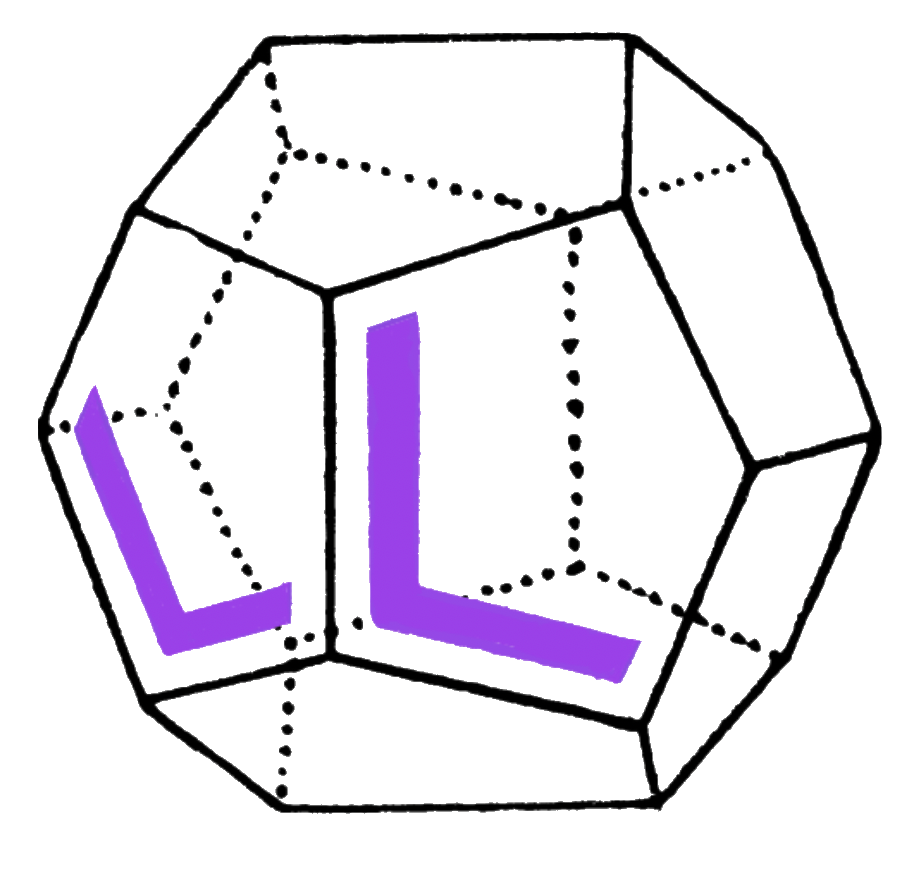
\includegraphics[width=2cm,height=2cm]{ll.png}}

    }}

\AddToShipoutPicture*
  {\put(470,737){

    \href{http://www.linearlibrary.net/CategoryTheory.pdf}{\texttt{.pdf file}}\\

  }}

\AddToShipoutPicture*
  {\put(470,752){
    \href{https://github.com/linlib/CategoryTheory/CategoryTheory.tex}{\texttt{.tex file}}\\

  }}

\AddToShipoutPicture*
  {\put(470,767){
    \href{http://www.linearlibrary.net/CategoryTheory/CategoryTheory.py}{\texttt{.py file}}

  }}

\AddToShipoutPicture*
  {\put(470,737){

    \href{https://github.com/linlib/CategoryTheory/CategoryTheory.pdf}{\texttt{.pdf file}}\\

  }}



\pagecolor{white}

\ \\
\ \\


\thispagestyle{empty} 

\AddToShipoutPicture*
    {\put(540,720){

    \href{http://www.linearlibrary.net}{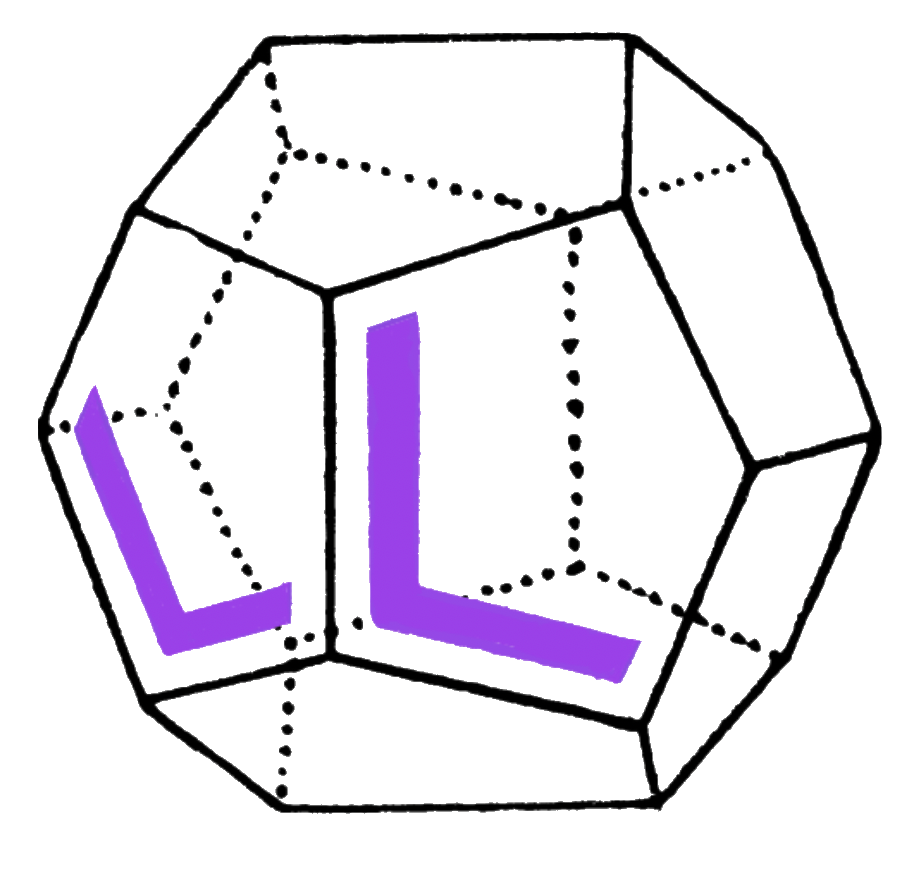
\includegraphics[width=2cm,height=2cm]{ll.png}}

    }}

\AddToShipoutPicture*
  {\put(470,767){
    \href{https://github.com/linlib/ThreeWhiteheadTheorems/StringDiagramGenerator.py}{\texttt{.py file}}
  }}

\AddToShipoutPicture*
  {\put(470,752){
    \href{https://github.com/linlib/ThreeWhiteheadTheorems/ThreeWhiteheadTheorems.tex}{\texttt{.tex file}}\\

  }}


\AddToShipoutPicture*
  {\put(470,737){

    \href{http://linearlibrary.net/ThreeWhiteheadTheorems/October19th.pdf}{\texttt{.pdf file}}\\

  }}

  \AddToShipoutPicture*
  {\put(470,722){
    \href{https://github.com/linlib/ThreeWhiteheadTheorems/ThreeWhiteheadTheorems.lean}{\texttt{.lean file}}

  }}

\ \\

%LEAN: 
\begin{center}
  \begin{tcolorbox}[width=3.5in,colback={white},coltitle=white]
  \begin{center}
  \ \\
  \scalebox{2}{\texttt{Internal Universes}}
  \ \\
  \end{center}
  \end{tcolorbox}
  \end{center}
  \ \\

{\footnotesize
\begin{center}
\scalebox{1.1}{
\begin{tabular}{|| l | l || l | l ||} 
\hline
$\texttt{∞\_(∞-Cat)}$   &  $\texttt{D(∞\_(∞-Cat))}$  & $\texttt{∞\_(∞-Cat)⁄C}$    & $\texttt{D(∞\_(∞-Cat)⁄C)}$\\
\hline
$\texttt{∞\_(∞-Grpd)}$  &  $\texttt{D(∞\_(∞-Grpd))}$  & $\texttt{∞\_(∞-Grpd)⁄G}$    & $\texttt{D(∞\_(∞-Grpd)⁄G)}$ \\
 \hline
$\texttt{∞\_(∞-Grpd₀)}$ &  $\texttt{D(∞\_(∞-Grpd₀))}$  & $\texttt{∞\_(∞-Grpd₀)⁄G₀}$  & $\texttt{D(∞\_(∞-Grpd₀)⁄G₀)}$ \\
 \hline
\end{tabular}}
\end{center}}
  


\newpage


\thispagestyle{empty}


\newpage
\section{Introduction}

In this repository I would like to consider Kan extensions and homotopy Kan extensions, obtaining a thorough account of Lurie's straightening and unstraightening concepts.\\



\newpage
\section{Unicode}

Here is a list of the unicode characters I will use:

{\footnotesize
\begin{center}
\begin{tabular}{|| l || l || l || l ||} 
\hline
$\texttt{Symbol}$ & $\texttt{Unicode}$ & \texttt{VSCode shortcut} & $\texttt{Use}$\\
\hline
\hline
\multicolumn{4}{||c||}{\texttt{Lean's Kernel}} \\
\hline
\hline
× & 2A2F & \backslash\texttt{times} & Product of types\\
\hline
→ & 2192 & \backslash\texttt{rightarrow}  & Hom of types\\
\hline
⟨,⟩ & 27E8,27E9 & \backslash\texttt{langle},\backslash\texttt{rangle}  & Product term introduction\\
\hline
↦ & 21A6 &\backslash\texttt{mapsto}  & Hom term introduction\\
\hline
∧ & 2227 &\backslash\texttt{wedge}  & Conjunction \\
\hline
∨ & 2228 &\backslash\texttt{vee}  & Disjunction \\
\hline
∀ & 2200 &\backslash\texttt{forall}  & Universal quantification \\
\hline
∃ & 2203 &\backslash\texttt{exists}  & Existential quantification\\
\hline
¬ & 00AC &\backslash\texttt{neg}  & Negation\\
\hline
\hline
\multicolumn{4}{||c||}{\texttt{Variables and Constants}} \\
\hline
\hline
ᵃ,ᵇ,ᶜ,...,ᶻ & 1D52,1D56 &\iffalse\backslash{}^{$\wedge$}\texttt{a},{\backslash{}}^{$\wedge$}\texttt{b},\backslash{}^{$\wedge$}\texttt{c},...\backslash{}^{$\wedge$}\texttt{z}\fi  & Variables and constants \\
\hline
⁰,¹,²,³,⁴,⁵,⁶,⁷,⁸,⁹ & 1D52,1D56 & \iffalse\backslash\wedge\texttt{0},\backslash{}^{$\wedge$}\texttt{1},\backslash{}^{$\wedge$}\texttt{2},...,\backslash{}^{$\wedge$}\texttt{9}\fi  & Variables and constants \\
\hline
⁻ & 207B & \iffalse\backslash\wedge\texttt{-},\fi  & Variables and constants \\
\hline
₀,₁,₂,₃,₄,₅,₆,₇,₈,₉ & 2080 - 2089 & \backslash\texttt{0}-\backslash\texttt{9} & Variables and constants\\
\hline
𝔸,...,ℤ & 1D538 & \backslash\texttt{bbA},...,\backslash\texttt{bbZ} &  Variables and constants \\
\hline
𝕒,...,𝕫 & 1D552 & \backslash\texttt{bba},...,\backslash\texttt{bbz} & Variables and constants \\
\hline
\iffalse 𝐀,...,𝐙 & 1D41A & \backslash\texttt{bfA},...,\backslash\texttt{bfZ} & Variables and constants \\
\hline
𝐚,...,𝐳 & 1D41A & \backslash\texttt{bfa},...,\backslash\texttt{bfz} & Variables and constants \\
\hline \fi
\texttt{α}-\texttt{ω},\texttt{A}-\texttt{Ω} & 03B1-03C9 & & Variables and constants\\
\hline
\hline
\multicolumn{4}{||c||}{\texttt{Categories and Bicategories}} \\
\hline
\hline
 𝟙 & 1D7D9 & \backslash\texttt{b1}  & The identity morphism\\
\hline
 ≫ & 2218 & & Composition\\
\hline
   &  &  & Composition\\
\hline
   &  &  & Composition\\
\hline
 \multicolumn{4}{||c||}{\texttt{Adjunctions}} \\
\hline
\hline\iffalse
⇄ & 21C4 & \backslash\texttt{rightleftarrows}  & Adjunctions \\
\hline
⇆ & 21C6 & \backslash\texttt{leftrightarrows}  & Adjunctions \\
\hline\fi
𛲔 & 1BC94 &  & Right adjoints\\
\hline
ॱ & 0971 &  & Left adjoints \\
\hline
⊣ & 22A3 & \backslash\texttt{dashv}  & The condition that two functors are adjoint \\
\hline
\hline
\multicolumn{4}{||c||}{\texttt{Monads and Comonads}} \\
\hline
\hline
?,¿ & 003F, 00BF & ?,\backslash\texttt{?}  & The corresponding (co)monad of an adjunction\\
\hline
!,¡ & 0021, 00A1 & !, \backslash\texttt{!}  & The (co)-Eilenberg-(co)-Moore adjunction \\
\hline
ꜝ,ꜞ & A71D, A71E &  & The (co)AdjMon maps\\
\hline
\hline
\multicolumn{4}{||c||}{\texttt{Miscellaneous}} \\
\hline
\hline
\iffalse ∼ & 223C & \backslash\texttt{sim} & Homotopies \\
\hline\fi
≃ & 2243 & \backslash\texttt{equiv}  & Equivalences \\
\hline
≅ & 2245 & \backslash\texttt{cong}   & Isomorphisms \\
\hline
⊥ & 22A5 & \backslash\texttt{bot}    & The overobject classifier \\
\hline
∞ & 221E & \backslash\texttt{infty}  & Infinity categories and infinity groupoids\\ 
 \hline
\end{tabular}
\end{center}}

Of these, the characters $\texttt{ꜝ,ꜞ,𛲔}$ and $\texttt{ॱ}$ do not have VSCode shortcuts, and so I provide alternatives for them. Possibly they will have to be changed if this work assimilates into a larger project.\\

It is not possible to copy the from the pdf to the clipboard while preserving the integrity of the code. To see the official Lean 4 file please click the link on the top right of the front page or \href{https://github.com/linlib/CategoryTheory/tree/main}{this}.



%LEAN: 
\begin{center}
\begin{tcolorbox}[width=5in,colback={white},title={\begin{center}\texttt{Lean \thelcounter} \addtocounter{lcounter}{1}  \end{center}},colbacktitle=Blue,coltitle=black]
\begin{minted}[breaklines, escapeinside=||]{lean}


import Mathlib.CategoryTheory.Bicategory.Basic
import Mathlib.CategoryTheory.Types 
import Mathlib.CategoryTheory.DiscreteCategory
import Mathlib.Combinatorics.Quiver.Basic
import Mathlib.CategoryTheory.Category.Init
import Aesop
import Init
import Mathlib.CategoryTheory.DiscreteCategory
import Mathlib.CategoryTheory.Bicategory.Strict
import Mathlib.CategoryTheory.ConcreteCategory.Bundled
import Mathlib.CategoryTheory.Functor.Basic
import Init.Core
import Mathlib.CategoryTheory.Category.Cat

import TheWhiteheadTheorem

-- #check 
-- #

\end{minted}
\end{tcolorbox}
\end{center}


\newpage
\begin{center}

\pagecolor{white}
\color{black}




\end{center}

\thispagestyle{empty}




\newpage
\pagecolor{white}
\color{black}
\ \\
\ \\
\thispagestyle{empty}
\begin{center}
Copyright\ \textcopyright \ June 2023 Elliot Dean Young.\ All rights reserved.\\
\end{center}
\large %%%%%%%% HERE IS THE large LARGE size textsize set text size
\newpage 
\ \\
\ \\
\ \\
\ \\
\ \\
\ \\
\ \\
\ \\
\ \\
\ \\
\ \\
\thispagestyle{empty}
 
\newpage
\section{Contents}

{
\footnotesize
\begin{longtable}{|| l || l ||} 
\hline
\multicolumn{1}{||c||}{$\texttt{Section}$} & \multicolumn{1}{|c||}{$\texttt{Description}$} \\
\hline
\hline
Unfinished & \\
\hline
Contents & \\
\hline
Unicode & \\
\hline
Introduction & \\
\hline \hline
\multicolumn{2}{||c||}{\texttt{PART I: } Internal Universes} \\
\hline \hline
\multicolumn{2}{||c||}{\texttt{Chapter 1: } ∞\_(∞-Cat)} \\
\hline \hline
χ⃗𛲔 : & \\
\hline 
χ⃗ॱ &  \\
\hline
D(χ⃗𛲔) &  \\
\hline
D(χ⃗ॱ) &  \\
\hline
D(∞$\_$(∞-Grpd₋₁)⁄-) &  \\
\hline
D([-ᵒᵖ,∞$\_$(∞-Grpd₋₁)]) &  \\
\hline
D(∞\_(∞-Grpd₋₁)⁄-) ≃ D([-ᵒᵖ,∞\_(∞-Grpd₋₁)]) &  \\
\hline \hline
\multicolumn{2}{||c||}{\texttt{Chapter 2: } ∞\_(∞-Grpd)} \\
\hline \hline
χ⃡𛲔 & \\
\hline
χ⃡ॱ & \\
\hline
D(χ⃡𛲔) & \\
\hline
D(χ⃡ॱ) & \\
\hline
D(∞\_(∞-Grpd)⁄-) & \\
\hline
\iffalse D([-ᵒᵖ,∞\_(∞-Grpd)]) \fi & \\
\hline
\iffalse D(∞\_(∞-Grpd)⁄-) ≃ D([-ᵒᵖ,∞\_(∞-Grpd)]) \fi & \\
\hline \hline
\multicolumn{2}{||c||}{\texttt{Chapter 3: } ∞\_(∞-Grpd₀)} \\
\hline \hline
χ𛲔 & \\
\hline
χॱ & \\
\hline
D(χ𛲔) & \\
\hline
D(χॱ) & \\
\hline
D(∞\_(∞-Cat)⁄-) & \\
\hline
D([-ᵒᵖ,∞\_(∞-Cat)]) & \\
\hline
D(∞\_(∞-Cat)⁄-) ≃ D([-ᵒᵖ,∞\_(∞-Cat)]) & \\
\hline
\end{longtable}
}


\iffalse
The way in which γ⃗ and γ⃡ are irreducible is governed by the ??? theorem in the repository concerning internal universes.\\

\fi



\part{Constructing Three Internal Universes}


\chapter{∞\_(∞-Grpd₀)}




\chapter{∞\_(∞-Grpd)}



\chapter{∞\_(∞-Cat)}




\iffalse

\iffalse
RedPRL
redtt
yacctt
cubicaltt
Agda

Carlo Angiuli, Guillaume Brunerie, Thierry Coquand, Kuen-Bang Hou (Favonia), Robert Harper, and Daniel R. Licata
Jonathan Sterling, Carlo Angiuli, Daniel Gratzer,
\fi

\iffalse
For the Whitehead theorem paper:

https://mail.google.com/mail/u/1/#search/reihl/CllgCJlHnCFvnhQdHXccDGWvDvgZXhGGLRcFsHnrxKBcrTQdfQVMZXpDTLBfcGdtnjWcZhrgfcL

https://www.math.uwo.ca/faculty/kapulkin/seminars/hottestfiles/Kudasov-2023-10-05-HoTTEST.pdf

Could demonstrate that the paper here is also a model of our theorems in a broader context, featuring extensionalities which are not available in RZK:

https://scholar.google.com/citations?user=n9Uqm4wAAAAJ&hl=en

https://arxiv.org/pdf/1705.07442.pdf

https://arxiv.org/pdf/2202.13132.pdf

- synthetic

In the last years, formalization of mathematics has caught the attention of an in- creasing number of mathematicians. The process of formalizing typically starts with mathematical definitions, theorem statements and proofs stated in natural language, proverbially written with pen and paper. Then, each step is made precise enough to ensure the full development is unambiguously and completely verifiable. Finally, the resulting precise steps are translated to produce a document written in a formal language. The process is complete when software can read this document and cer- tify that the formal development has no logical errors or omissions. Formalization requires a formalism, a system of logic that can decide which steps are allowed and which cause errors.
This thesis concerns formalization of mathematics in the Lean theorem prover [90], as part of the Mathlib library [117].1 Lean is an example of an interactive theorem prover (ITP) or proof assistant, a program allowing users to perform precise and verified mathematical reasoning on the computer. Lean is an interactive theorem prover because the user is expected to enter a proof themself in the formal language, guided interactively by the software reporting proof progress in response to typed commands, so in turn the user can type new commands in response to the proof state. The proof state includes a list of available hypotheses and unproved goals, and any logical errors that Lean has detected. Working interactively in this way involves a specialized or extended text editor2 that shows the state of the proof assistant and updates dynamically as the user types or moves through documents.
In contrast, automated theorem provers search autonomously for a proof, given a theorem statement. The output of automated theorem provers has been used with success as ingredients of a solution to open mathematical problems [65, 73, 83], but it appears we are still far away from completely automating the insights that were needed to translate these specific conjectures to a form the computer can solve, let alone figure out how to do so for any given conjecture. Human interaction will be needed for computer proving for the foreseeable future.
The division between automated and interactive provers is not absolute. There are hammers, tools that use the output of automated theorem provers to build interactive proofs [42, 71, 102]. Moreover, all generally used interactive theorem provers offer a variety of more specific automation tools that relieve the user from having to break down every proof to the lowest-level logical deduction rules. Still, the formalizer has to be much more explicit about details that can be safely left out in pen and paper mathematics.
If interactive theorem proving requires extra work, why not stick to pen and paper? A simple answer is: it is fun to work with an interactive theorem prover, since collaborating on a library of formal mathematics is in a way the ultimate massively multiplayer online puzzle video game.3
More seriously, there are scientific motivations for formalizing mathematics. First of all, by writing mathematical statements in a formal language, software can verify and analyze the contents precisely. We can be very confident that a computer- verified proof has no mistakes, and verification is precisely what a proof assistant does with its input. While this certainty is a useful consequence of formalization, the added confidence is a requirement, rather than a bonus, only in rare (but no less interesting) cases. These include the formal verifications of the proofs of the Four Color Theorem [58], the Kepler Conjecture [63] and the main theorem of liquid vector
 1https://leanprover-community.github.io/lean3/ (accessed 2023-09-21)
2The editors supported by Lean are VS Code, Emacs and Neovim.
3Comparisons along these lines have been made many times by many people; the first instance I was
 able to track down was in a series of Semantics lectures given by Tobias Nipkow. 2
1.1. MOTIVATION   3
spaces [40]. On the other hand, I cannot imagine there is a serious mathematician who doubts that, for instance, the class group of the ring of integers of a number field is finite.
Still, the goal of verification can justify formalization of well understood results. A thorough coverage of existing work is required before we can embark on the verification of novel results, and often even before we have the language to state a theorem. To catch up with the thousands of years of mathematical development takes a significant amount of formalization effort. It is only in the last few years that the field of formalization has caught up enough that it is possible at all to formalize new results soon after they are announced. In particular, Thomas F. Bloom and Bhavik Mehta completed a formalization of a paper written by the former (and its dependencies) in about half a year, before the paper exited peer review [22, 23].
Outside of verification, applications have a more experimental character. In the field of machine learning, proof assistants have received attention because the ex- actness of formal reasoning counterbalances the heuristic and unvalidated mode of reasoning. Thus they can serve as a source of truth for training machine learning systems [16, 103, 104], or for verifying their output. While the interaction between interactive theorem provers and large language models is certainly an interesting avenue of research, this thesis is GPT-free.
Looking at more traditional algorithmic approaches to reasoning, the advantages brought by formalization are in the uniform and precise format used to present for- malized results, meaning various interesting properties of the work can be computed directly. For instance, there is a Lean metaprogram which can analyze whether the hypotheses in a theorem statement are unnecessarily strong for the given proof, and suggest a more general statement automatically [19].
The level of formality required in interactive theorem proving also contributes to human understanding. ITPs allow no excuses or hand-waving, so they provide the formalizer with a very specific list of what it does not “understand” (and therefore what the formalizer might not understand either). Implicit assumptions and modes of thinking become explicit objects when formalizing, and choosing a definition that formalizes better can guide the practitioner to learn new aspects of mathematics. The interactivity means near-instant feedback on any mistakes, accelerating the learning process. Finally, developing an interactive theorem prover provides a challenge for computer scientists, to make software understand human reasoning and communica- tion well enough that it can be easily translated to a formal language.
In addition to the research opportunities offered by interactive theorem proving in general, developing a large mathematical library throws up some interesting questions of its own. It is not obvious a priori that the heavily interdependent state of modern mathematics can fit without conflicts in one library. Given the variety of roles that each mathematical object is supposed to play, can we truly give a unique precise definition to each concept? A large library casting all of mathematics in a unified language and presentation could help provide a solid basis for education, or serve as a comprehensive reference.4 Alternatively, we can extract a natural language document from a formal development, with the formal results providing structure and details for the informal text [92]. On the computer science side, developing, maintaining and refactoring such a large library requires solving software engineering challenges in much the same way as any large software development project. These challenges are heightened by the global correctness constraints imposed by various features of the theorem prover.
The early landmark of interactive theorem proving for formal mathematics was Automath, developed under the leadership of De Bruijn [94]. Mizar, developed
4I am however not aware of a formal mathematical library designed for the purpose of teaching mathematics. Such a library would certainly look very different from the Lean mathematical library.

around the same time, is still in use nowadays [68, 93]. These early developments have been joined over time by a large array of proof assistants based on a wide variety of logical foundations. A relevant, but ultimately arbitrary, selection of ITPs that are in use for nontrivial mathematical formalizations consists of Agda, Coq, HOL Light, Isabelle/HOL, Metamath, Mizar and Lean. Since the systems differ in foundational logic and user interface, each prover has its own best practices and design patterns for formal developments to make optimal use of the proof language.
Lean is a relatively new addition to the set of proof assistants, but has rapidly gained a large dedicated community working on the Mathlib project, aiming to build one large library for all mathematical developments that can reasonably be supported, from the definition of the real numbers to the main theorem of liquid vector spaces. The decision of which prover and library to work with can be made on many grounds. Proof assistants have a variety of technical characteristics which can make them more suitable for specific areas of mathematics. Libraries similarly have differing design goals. Harder to make precise, but no less important, is the community around the prover, since developing a library of formal mathematics is a collaborative effort.
In the research I describe, my main focus was algebraic number theory, a central area of mathematics with classical roots that has been an essential ingredient in the resolution of famous problems such as Fermat's Last Theorem. The term “algebraic number theory” should be interpreted as the theory of algebraic numbers, which occur as elements of number fields, finite extensions of the field of rational numbers, and of algebraic integers that can be found in subrings of these number fields. Algebraic number theory is therefore a more specialized subject than the mere application of algebra to number theory that is suggested by the name. Its central and modern nature means algebraic number theory depends on developments in diverse areas of mathematics. A formalization of this area therefore serves as a good check that the definitions from these disparate fields work well together without the usual implicit identifications of informal reasoning. Moreover, despite previous formalizations of specific rings and fields of algebraic numbers, the general foundations underlying algebraic number theory had not been formalized in depth before, and Mathlib's existing strengths in algebra made the start accessible.


2.1 Reading Lean code
The formal system of Lean [34] is a dependent type theory in the Martin-Löf tra- dition [82] based on the calculus of inductive constructions [101]. The foundations of Lean closely resemble those of Coq [116]. In dependent type theory, each math- ematical object, represented by a term e, is an element of a unique type t, written e : t. The natural number 0 has type N, and the rational number 0 has type Q. The question whether the natural number 0 : N equals the rational number 0 : Q is not type-correct, unless one first maps 0 : N to Q. Lean will automatically insert such a map N → Q called a coercion and denoted by the arrow↑, that is,(0 : Q) = ↑(0 : N) (Section 3.3).
Dependent type theory blurs the distinction between types and terms. Thus, types have types too, for example N : Type. In technical terms, the full hierarchy in Lean consists of an impredicative universe Prop sitting at the bottom of a noncumulative chain Prop : Type : Type 1 : Type 2 : ...; “an arbitrary Type u” is abbreviated as Type* and “either Prop or Type*” is abbreviated Sort*. Propositions, i.e. statements that can be assigned a truth value, correspond to elements of Prop, while a (verified) proof of the proposition P : Prop corresponds to an element p : P. Thus checking the correctness of a proof becomes equivalent to verifying a term is well-typed.
The fact that Prop is impredicative means here that it is possible to quantify over all elements of any Sort* inside of the Prop universe. For example, the statement that each proposition is either true or false can be written as the term:
(∀ (P : Prop), P = true ∨ P = false) : Prop
In contrast, the Type* universes are not impredicative, so for instance we have:
1https://github.com/gebner/trepplein (accessed 2023-09-21) 8
 
2.1. READING LEAN CODE 9
(∀ (P : Type), P ≃ unit ⊕ P ≃ empty) : Type 1
 (recalling that Type is one universe level below Type 1). Universes in Lean are not cumulative, meaning that every type belongs to exactly one universe, and an explicit plift : Sort u → Sort (u + 1) operation must be inserted to increase the universe level. Lifting universe levels would quickly become cumbersome, so definitions themselves are also made universe parametric, which we can interpret as a copy of each definition existing in every sufficiently large universe. In practice universe issues are rare, and we can almost everywhere hide explicit reasoning about universe levels behind the notation Type*.
In addition to the mentioned features, commonly found in a dependent type the- ory, Lean provides, and Mathlib uses, proof irrelevance, quotient types and classical reasoning. Proof irrelevance means that for any proposition P : Prop, any two proofs p1 p2 : P are judged equal by the system (Section 2.4). Quotient types allow equiva- lence relations to be lifted to become actual equalities (Section 2.4). Classical reasoning in Lean takes the form of applying a type-theoretic axiom of choice, without which the system would be intuitionistic (Section 2.1.1).
Lean and Mathlib attempt to write terms that closely resemble common mathemat- ical notation. Following typical practice in logic, the conjunction of two propositions P Q : Prop is written P ∧ Q : Prop, disjunction is written P ∨ Q : Prop and impli- cation is written P → Q : Prop. The arrow symbol → is used both for implication between propositions and for functions between types: recall the coercion of type N → Q.
The notations used for functions are based on the λ calculus and should be somewhat familiar to functional programmers. To denote a function that squares its argument, we write λ x, x * x. Function application in Lean is written by juxtaposi- tion, so a function f applied to the argument x is written f x. Functions with multiple arguments are curried, meaning that the binary addition operator (+) : N → N → N is actually a function taking some a : N and returning a partially applied function (+) a : N → N.
The reuse of → is not just a syntactic convenience but reflects an identification of the two concepts in dependent type theory. We can view a proof of the impli- cation P → Q as a function transforming proofs of P into proofs of Q, known as the Brouwer-Heyting-Kolmogorov interpretation of implication [119]. Functions and impli- cations are examples of Π types, or dependent products, which have the general form Π(x:A),Bx, whereAandBxhave typeSort*. The notationA→Bis the same as the typeΠ(x:A),BwhereBdoes not depend onx:A. A third role played by Π types is that of universal quantification: a predicate on a type A is denoted by a function P : A → Prop, and to show P is true on every element of A simultaneously, we can give an element of Π (x : A), P x. The symbol ∀ is available as a synonym of Π to make the denotation clearer: ∀ (x : A), P x.
The sorry keyword can be used as a placeholder for a term. Any declaration using sorry will report an error when it is checked. Since sorry can be used in the place of any term, even in inconsistent contexts, it serves as an “escape hatch” for creating syntactically correct examples of erroring declarations. This thesis also uses sorry to hide irrelevant aspects of the full code that would take up too much space to show in full. All of the omitted code is available in full (and free of sorry) in the verified source code.
A Lean file is structured as a sequence of declarations, that correspond broadly to the definitions and theorems of a natural language mathematical document. In general, a declaration consists of a keyword, a name, a list of parameters, a term denoting the type and a term denoting the value. For example, the declaration below has keyword def, name square, parameter list (x : R), type R and value x * x.
defsquare(x: R): R :=x*x
9

10   CHAPTER 2. LEAN AND MATHLIB
Every declaration is checked to ensure it is consistent with Lean's logic; in particular the type of the value should match the declared type. Subsequent declarations can then use the name square to refer to the function that maps x : R to its square. Specifically, square is a term of type Π (x : R), R and value λ (x : R), x * x, so the type and value we write down in a declaration are combined with the parameters to specify the type and value of the corresponding term.
The simplest declaration keywords in Lean are theorem, lemma and def. There is no distinction between theorem and lemma in the formal system; these merely serve to guide the (human) reader. Like def, the theorem keyword allows subsequent declarations to use a term named in the theorem declaration. However, the value of a theorem (which represents a proof of that theorem) is not available in Lean beyond checking the declaration, so it does not play a role in definitional equality checking (Section 2.4). Therefore, theorems are used for proofs living in the Prop universe where the specific value does not matter (due to proof irrelevance). Lean has many more declaration keywords that will be explained as they appear in this thesis.
2.1.1 Classical reasoning in Lean
Martin-Löf type theory and the calculus of inductive constructions were originally designed to serve as foundations for constructive mathematics. Lean extends these constructive foundations with the axiom classical.choice:
axiom classical.choice {α : Sort u} : nonempty α → α
Here, the proposition nomempty α : Prop is empty whenever α is empty and has ex- actly one element if α has at least one element. In homotopy type theory terms, nonempty is the propositional truncation operator. This axiom is analogous to introduc- ing the double negation elimination proof rule ¬¬ p → p. The name classical.choice reflects its status in type theory as a generalization of the set theoretical axiom of choice, which is included in Lean as a corollary of the type theoretical choice principle:
theorem classical.axiom_of_choice (h : ∀ x, ∃ y, r x y) : ∃ f, ∀ x, r x (f x)
Specifically, Diaconescu's theorem states that the principle of excluded middle can be derived from classical.choice together with function extensionality and propo- sitional extensionality. Function extensionality is a theorem in Lean's foundations, provable from the existence of quotient types (Section 2.4), while propositional ex- tensionality is an axiom:
axiom propext {a b : Prop} : (a ↔ b) → a = b
Mathlib follows common mathematical practice and makes use of classical rea- soning throughout the library, with very specific exceptions. Lean provides a type decidable (p : Prop) : Type, intended for propositions that can be shown construc- tively to satisfy the principle of excluded middle. This is applied in proof automation: dec_trivial is a procedure that attempts to prove a proposition p by searching for a suitable value of decidable p and checking that the decision algorithm indeed shows the proposition is true. Apart from this section, intuitionistic reasoning plays no important role in the thesis, and we will only use the word ``classical'' to mean an established and important result.

"actually worked as an assistant"
- Id₁, Id₂, Ass
\fi



\section{Lan D(∞-Cat)}


\iffalse

[-,∞-Cat]
[-,∞-Grpd]
[-,∞-Grpd₀]


[-,∞-Cat]
[-,∞-Grpd]
[-,∞-Grpd₀]

\fi


\chapter{ETCC Signature 3}

ETCC signature 3 says that 

\begin{enumerate}
\item D(∞\_(∞-Cat)) classifies D(∞\_(∞-Cat)⁄-) : ∞\_(∞-Cat) ⭢ ∞\_(∞-Cat)
\item 
\end{enumerate}





\iffalse

\chapter{Chapter 2: Pullback Systems} 

\section{$\texttt{pullback\_systems}$}
$\texttt{pullback\_systems}$ is a type defined in this kernel to handle derived directed homotopy pullback and directed homotopy pullback of something with itself (which we take to be directed path space [Δ1,-]). It also stores the information of the category D(∞-Cat), as well as D(∞-Cat⁄C) for each C : D(∞-Cat). D(∞-Cat) has a universe object ∞ as well, and a point *, and a map ⊥ : * → ∞. Various constructions associated to ∞-categories with a kind of universe object form the only example of a pullback system that we will use here, and yet it may prove to be useful in understanding how to force a situation in which the Whitehead theorem applies later on. \\
%LEAN: defining a pullback system
\begin{center} \begin{tcolorbox}[width=5in,colback={white},title={\begin{center}\texttt{Lean \thelcounter} \addtocounter{lcounter}{1} \end{center}},colbacktitle=Blue,coltitle=black] \begin{minted}[breaklines, escapeinside=||]{lean}

 /-
structure pullback_system where
Obj : Cat
Pnt : Obj
CmpObj : Obj.Obj → Cat CmpHom : (C : Obj.Obj) →
(D : Obj.Obj) →
(F : Obj.Hom C D) → (Functor (CmpObj C) (CmpObj D)) -- note this may need tweaking, but it should produce a functor F : D(∞-Cat/D) → D(∞-Cat/C) for each
--
CmpIdn : (C : Obj.Obj) → ((CmpHom C C (𝟙_(Obj) C)) = 𝟏_(𝐂𝐚𝐭) (CmpObj C)) CmpCmp : (C : Obj.Obj) → (D : Obj.Obj) → (E : Obj.Obj) → (F : Obj.Hom C D) → (G :
Obj.Hom D E) → (((CmpHom D E G) •_(𝐂𝐚𝐭) (CmpHom C D F)) = CmpHom C E (G ∘_(Obj) F))
Fix : Obj ≃_(𝐂𝐚𝐭) (CmpObj Pnt) Pul : (C : Obj.Obj) →
(D : Obj.Obj) →
(F : Obj.Hom C D) →
(𝐂𝐚𝐭.Hom (CmpObj D) (CmpObj C)).Obj
η : (C : Obj.Obj) → (D : Obj.Obj) → (F : Obj.Hom C D) → ((𝐂𝐚𝐭.Hom (CmpObj C) (CmpObj C)).Hom (𝟏_(𝐂𝐚𝐭) (CmpObj C)) ((Pul C D F) •_(𝐂𝐚𝐭) (CmpHom C D F)))
ε : (C : Obj.Obj) → (D : Obj.Obj) → (F : Obj.Hom C D) → ((𝐂𝐚𝐭.Hom (CmpObj D) (CmpObj D)).Hom ((CmpHom C D F) •_(𝐂𝐚𝐭) (Pul C D F)) (𝟏_(𝐂𝐚𝐭) (CmpObj D)))
Id1 : (C : Obj.Obj) → (D : Obj.Obj) → (F : Obj.Hom C D) → (AdjId1 𝐂𝐚𝐭 (CmpObj C) (CmpObj D) (CmpHom C D F) (Pul C D F) (η C D F) (ε C D F))
Id2 : (C : Obj.Obj) → (D : Obj.Obj) → (F : Obj.Hom C D) → (AdjId2 𝐂𝐚𝐭 (CmpObj C) (CmpObj D) (CmpHom C D F) (Pul C D F) (η C D F) (ε C D F))
Inf : Obj.Obj
Ovr : Obj.Hom Pnt Inf
Chi : (C : Obj.Obj) → (F : (CmpObj C).Obj) → ((Obj.Hom) C Inf)
-- ??? : (C : Obj.Obj) → (F : (Cmp C).Obj) → ((Pul C Inf (χ C f)).Hom Pnt Inf Ovr = f) -/
\end{minted} \end{tcolorbox} \end{center}
The last axiom above is a bit tricky, but it is related to straightening and unstraightening.\\ We use the notation like this:
%LEAN:

 \begin{center} \begin{tcolorbox}[width=5in,colback={white},title={\begin{center}\texttt{Lean \thelcounter} \addtocounter{lcounter}{1} \end{center}},colbacktitle=Blue,coltitle=black] \begin{minted}[breaklines, escapeinside=||]{lean}
notation "D(" Γ "⁄-)" => "Γ"
\end{minted} \end{tcolorbox} \end{center}
In the remainder of this section, I made some boxes which altogether filled out make pullback systems into a category.\\
%LEAN: defining a map of pullback systems
\begin{center} \begin{tcolorbox}[width=5in,colback={white},title={\begin{center}\texttt{Lean \thelcounter} \addtocounter{lcounter}{1} \end{center}},colbacktitle=Blue,coltitle=black] \begin{minted}[breaklines, escapeinside=||]{lean}
-- defining a map of pullback systems
structure PulHom (Γ1 : pullback_system) (Γ2 : pullback_system) where
Obj : (𝐂𝐚𝐭.Hom Γ1.Obj Γ2.Obj).Obj
Obj2 : (C : Γ1.Obj.Obj) → (𝐂𝐚𝐭.Hom (Γ1.CmpObj C) (Γ2.CmpObj (Obj.Obj C))).Obj -- plays well with CmpHom?
-- Idn
-- Cmp
\end{minted} \end{tcolorbox} \end{center}
%LEAN: defining the identity map of two pullback systems
\begin{center} \begin{tcolorbox}[width=5in,colback={white},title={\begin{center}\texttt{Lean \thelcounter} \addtocounter{lcounter}{1} \end{center}},colbacktitle=Blue,coltitle=black] \begin{minted}[breaklines, escapeinside=||]{lean}
-- defining the identity map of two pullback systems def PulIdn (X : pullback_system) : PulHom X X := sorry
\end{minted} \end{tcolorbox}

 \end{center}
%LEAN: defining the composition of two pullback systems
\begin{center} \begin{tcolorbox}[width=5in,colback={white},title={\begin{center}\texttt{Lean \thelcounter} \addtocounter{lcounter}{1} \end{center}},colbacktitle=Blue,coltitle=black] \begin{minted}[breaklines, escapeinside=||]{lean}
-- defining the composition of two pullback systems
def PulCmp (X : pullback_system) (Y : pullback_system) (Z : pullback_system) (_ : PulHom X Y) (_ : PulHom Y Z) : PulHom X Z := sorry
\end{minted} \end{tcolorbox} \end{center}
%LEAN: proving the first identity law for maps of pullback systems
\begin{center} \begin{tcolorbox}[width=5in,colback={white},title={\begin{center}\texttt{Lean \thelcounter} \addtocounter{lcounter}{1} \end{center}},colbacktitle=Blue,coltitle=black] \begin{minted}[breaklines, escapeinside=||]{lean}
-- proving the first identity law for maps of pullback systems
def PulId1 (X : pullback_system) (Y : pullback_system) (f : PulHom X Y) : PulCmp X Y Y f (PulIdn Y) = f := sorry
\end{minted} \end{tcolorbox} \end{center}
%LEAN: proving the second identity law for maps of pullback systems
\begin{center} \begin{tcolorbox}[width=5in,colback={white},title={\begin{center}\texttt{Lean \thelcounter} \addtocounter{lcounter}{1} \end{center}},colbacktitle=Blue,coltitle=black] \begin{minted}[breaklines, escapeinside=||]{lean}
-- proving the first identity law for maps of pullback systems
def PulId2 (X : pullback_system) (Y : pullback_system) (f : PulHom X Y) : PulCmp X X Y (PulIdn X) f = f := sorry
\end{minted}

 \end{tcolorbox} \end{center}
%LEAN: proving the associativity law for maps of pullback systems
\begin{center} \begin{tcolorbox}[width=5in,colback={white},title={\begin{center}\texttt{Lean \thelcounter} \addtocounter{lcounter}{1} \end{center}},colbacktitle=Blue,coltitle=black] \begin{minted}[breaklines, escapeinside=||]{lean}
def PulAss (W : pullback_system) (X : pullback_system) (Y : pullback_system) (Z : pullback_system) (f : PulHom W X) (g : PulHom X Y) (h : PulHom Y Z) : PulCmp W X Z f (PulCmp X Y Z g h) = PulCmp W Y Z (PulCmp W X Y f g) h := sorry
\end{minted} \end{tcolorbox} \end{center}
%LEAN: constructing the category Pul of pullback systems
\begin{center} \begin{tcolorbox}[width=5in,colback={white},title={\begin{center}\texttt{Lean \thelcounter} \addtocounter{lcounter}{1} \end{center}},colbacktitle=Blue,coltitle=black] \begin{minted}[breaklines, escapeinside=||]{lean}
-- constructing the category Pul of pullback systems
def Pul : category := {Obj := pullback_system, Hom := PulHom, Idn := PulIdn, Cmp := PulCmp, Id1 := PulId1, Id2 := PulId2, Ass := PulAss}
notation "Loc" => Pul
\end{minted} \end{tcolorbox} \end{center}
\section{The Pullback System of Infinity Categories}
The pullback system will be able to encapsulate information associated to ∞-Cat, D(∞-Cat),
and D(∞-Cat⁄C), namely the derived directed homotopy pullback functor and its adjoint D(ω𛲔.hom f), derived postcomposition D(ωॱ.hom f).\\
$D(Γ)$ is the ``Obj" component from the above structure: %LEAN:

 \begin{center} \begin{tcolorbox}[width=5in,colback={white},title={\begin{center}\texttt{Lean \thelcounter} \addtocounter{lcounter}{1} \end{center}},colbacktitle=Blue,coltitle=black] \begin{minted}[breaklines, escapeinside=||]{lean}
def D (Γ : pulback_system) := Γ.Obj
\end{minted} \end{tcolorbox} \end{center}
Meanwhile, the categories $D($∞$-Cat⁄C)$ are formed from the the $\texttt{CmpObj}$ components in the above like this:
%LEAN:
\begin{center} \begin{tcolorbox}[width=5in,colback={white},title={\begin{center}\texttt{Lean \thelcounter} \addtocounter{lcounter}{1} \end{center}},colbacktitle=Blue,coltitle=black] \begin{minted}[breaklines, escapeinside=||]{lean}
def derived_category (Γ : pullback_system) (C : Γ.Obj.Obj) : 𝐂𝐚𝐭.Obj := Γ.CmpObj C
\end{minted} \end{tcolorbox} \end{center}
%LEAN:
\begin{center} \begin{tcolorbox}[width=5in,colback={white},title={\begin{center}\texttt{Lean \thelcounter} \addtocounter{lcounter}{1} \end{center}},colbacktitle=Blue,coltitle=black] \begin{minted}[breaklines, escapeinside=||]{lean}
-- notation "Cmp_(" Γ ")" => derived_category Γ notation "D(" Γ "⁄" C ")" => derived_category Γ C
\end{minted} \end{tcolorbox} \end{center}
\section{$\texttt{ω⃗\_(Γ) f}$}

 Each pullback system features a construction ω⃗ which is the directed homotopy pullback in the case of ∞-categories.\\
%LEAN: assembling the adjunction ω⃗_(Γ)
\begin{center} \begin{tcolorbox}[width=5in,colback={white},title={\begin{center}\texttt{Lean \thelcounter} \addtocounter{lcounter}{1} \end{center}},colbacktitle=Blue,coltitle=black] \begin{minted}[breaklines, escapeinside=||]{lean}
def directed_homotopy_pullback (Γ : pullback_system) (E : Γ.Obj.Obj) (B : Γ.Obj.Obj) (f : Γ.Obj.Hom E B) : (adjunction 𝐂𝐚𝐭) := sorry
\end{minted} \end{tcolorbox} \end{center}
%LEAN: notation for ω⃗_(Γ)
\begin{center} \begin{tcolorbox}[width=5in,colback={white},title={\begin{center}\texttt{Lean \thelcounter} \addtocounter{lcounter}{1} \end{center}},colbacktitle=Blue,coltitle=black] \begin{minted}[breaklines, escapeinside=||]{lean}
notation : 4000 "ω⃗_(" Γ ")" => pullback Γ
\end{minted} \end{tcolorbox} \end{center}
%LEAN: (ω⃗_(Γ) 𝟙_(?) C)𛲔 = 𝟏_(?) (ω⃗_(Γ) C)𛲔
\begin{center} \begin{tcolorbox}[width=5in,colback={white},title={\begin{center}\texttt{Lean \thelcounter} \addtocounter{lcounter}{1} \end{center}},colbacktitle=Blue,coltitle=black] \begin{minted}[breaklines, escapeinside=||]{lean}
--
/-
def pIdn : -/
\end{minted} \end{tcolorbox} \end{center}

 %LEAN: (ω⃗_(Γ) f)𛲔 •_(?) (ω⃗_(Γ) g)𛲔 = (p_(Γ) f ∘_(?) g)𛲔
\begin{center} \begin{tcolorbox}[width=5in,colback={white},title={\begin{center}\texttt{Lean \thelcounter} \addtocounter{lcounter}{1} \end{center}},colbacktitle=Blue,coltitle=black] \begin{minted}[breaklines, escapeinside=||]{lean}
--
/-
def pCmp : -/
\end{minted} \end{tcolorbox} \end{center}
\section{$\texttt{*\_(Γ)}$}
The terminal object is the $\texttt{Pnt}$ component, and will be pretty easy to fill out in our
upcoming semantics:
%LEAN:
\begin{center} \begin{tcolorbox}[width=5in,colback={white},title={\begin{center}\texttt{Lean \thelcounter} \addtocounter{lcounter}{1} \end{center}},colbacktitle=Blue,coltitle=black] \begin{minted}[breaklines, escapeinside=||]{lean}
-- def terminal_object (Γ : pullback_system) : Γ.Obj.α := Γ.Pnt
\end{minted} \end{tcolorbox} \end{center}
%LEAN:
\begin{center} \begin{tcolorbox}[width=5in,colback={white},title={\begin{center}\texttt{Lean \thelcounter} \addtocounter{lcounter}{1} \end{center}},colbacktitle=Green,coltitle=black] \begin{minted}[breaklines, escapeinside=||]{lean}
notation : 3000 "*_(" Γ ")" => terminal_object Γ
\end{minted} \end{tcolorbox}

 \end{center} \section{$\texttt{∞\_(Γ)}$}
The $\texttt{Inf}$ component is the internal universe in D(∞-Cat). I didn't mention this before since it's really tricky to get right in a way which doesn't encumber the approach.\\
%LEAN:
\begin{center} \begin{tcolorbox}[width=5in,colback={white},title={\begin{center}\texttt{Lean \thelcounter} \addtocounter{lcounter}{1} \end{center}},colbacktitle=Blue,coltitle=black] \begin{minted}[breaklines, escapeinside=||]{lean}
def universe_object (Γ : pulback_system) : Γ.Obj.Obj := Γ.Inf
\end{minted} \end{tcolorbox} \end{center}
%LEAN:
\begin{center} \begin{tcolorbox}[width=5in,colback={white},title={\begin{center}\texttt{Lean \thelcounter} \addtocounter{lcounter}{1} \end{center}},colbacktitle=Blue,coltitle=black] \begin{minted}[breaklines, escapeinside=||]{lean}
notation "∞_(" Γ ")" => universe_object Γ
\end{minted} \end{tcolorbox} \end{center}
\section{$\texttt{⊥\_(Γ)}$}
Here we define the "false" map, which consists of a point mapping into the universe object. Directed homotopy pullback of F : C → ∞\_(Γ) is of very special significance, and related to Lurie's ``straightening" and ``unstraightening".\\
%LEAN: defining ⊥_(Γ) : Γ.Obj.Hom *_(Γ) ∞_(Γ)
\begin{center} \begin{tcolorbox}[width=5in,colback={white},title={\begin{center}\texttt{Lean \thelcounter} \addtocounter{lcounter}{1} \end{center}},colbacktitle=Blue,coltitle=black] \begin{minted}[breaklines, escapeinside=||]{lean}

 -- defining ⊥_(Γ) : Γ.Obj.Hom *_(Γ) ∞_(Γ)
-- def overobject_classifier (Γ : pullback_system) (p: pullback_system Γ) : (Γ.Obj.Hom *_(Γ) ∞_(Γ)) := O.Ovr
\end{minted} \end{tcolorbox} \end{center}
%LEAN:
\begin{center} \begin{tcolorbox}[width=5in,colback={white},title={\begin{center}\texttt{Lean \thelcounter} \addtocounter{lcounter}{1} \end{center}},colbacktitle=Blue,coltitle=black] \begin{minted}[breaklines, escapeinside=||]{lean}
-- notation "⊥_(" Γ ")" => overobject_classifier Γ
\end{minted} \end{tcolorbox} \end{center}
\section{$\texttt{χ\_(Γ)}$}
The $\textit{straightening}$ of \texttt{χ.obj F : D → ∞\_(∞-Cat)} an ∞-functor F : C → D is an
object in ∞-Cat ⁄ C.
%LEAN: defining χ_(Γ) : ???
\begin{center} \begin{tcolorbox}[width=5in,colback={white},title={\begin{center}\texttt{Lean \thelcounter} \addtocounter{lcounter}{1} \end{center}},colbacktitle=Blue,coltitle=black] \begin{minted}[breaklines, escapeinside=||]{lean}
-- defining χ_(Γ) : ???
-- def straightening (Γ : pullback_system) {_ : overobject_classifier Γ}
\end{minted} \end{tcolorbox} \end{center}
%LEAN:
\begin{center}

 \begin{tcolorbox}[width=5in,colback={white},title={\begin{center}\texttt{Lean \thelcounter} \addtocounter{lcounter}{1} \end{center}},colbacktitle=Blue,coltitle=black] \begin{minted}[breaklines, escapeinside=||]{lean}
-- notation "χ_(" Γ ")" =>
\end{minted} \end{tcolorbox} \end{center}
The last two components of the pullback\_system strucuture (the very last of which is currently unfilled) ensure that straightening and unstraightening hold.\\
\chapter{Set}
We next produce the simplest example of a pullback system, namely $\texttt{𝕊𝕖𝕥}$, whose object component $\texttt{𝕊𝕖𝕥.Obj}$ is the category $\texttt{Set}$ previously constructed. It is the only example of a pullback system that we construct besides the main one.\\
I haven't filled any of this out, but it is much easier to see how set maps f : X → Y correspond to set maps Y → ∞\_(𝕊𝕖𝕥) than for the case of ∞-C𝕒𝕥 (which is the mentioned pullback system from which we will obtain such objects as D(∞-Cat/C) and D(∞-Cat).\\
Currently I don't have any of this filled out, but keep in mind that the analogue of ω⃗ here is simply pullback of sets (much simpler than directed derived directed homotopy pullback).\\
\chapter{Kan Extensions}
{\footnotesize \begin{center} \begin{tabular}{|| l || l ||}
\hline
$\texttt{Section}$ & $\texttt{Description}$ \\
\hline \hline
\texttt{[Cop,Set] ⇄ [Dop,Set]} & The left Kan extension \\ \hline
\texttt{[C,Set]op ⇆ [D,Set]op} & The right Kan extension \\ \hline

 \end{tabular} \end{center}} \\\
\\\
%LEAN:
\begin{center} \begin{tcolorbox}[width=5in,colback={white},title={\begin{center}\texttt{Lean \thelcounter} \addtocounter{lcounter}{1} \end{center}},colbacktitle=Blue,coltitle=black] \begin{minted}[breaklines, escapeinside=||]{lean}
-- def el (Γ : pullback_system) (C : D(Γ).Obj) (F : D(Γ).Hom C ∞_(Γ)) := (Γ.Pul C ∞_(Γ) F).Hom *_(Γ) ∞_(Γ) ⊥_(Γ)
-- #check el /-
-/
\end{minted} \end{tcolorbox} \end{center}
\section{\texttt{[Cop,∞-Cat] ⇄ [Dop,∞-Cat]}}
%LEAN: defining the left Kan extension on objects
\begin{center} \begin{tcolorbox}[width=5in,colback={white},title={\begin{center}\texttt{Lean \thelcounter} \addtocounter{lcounter}{1} \end{center}},colbacktitle=Blue,coltitle=black] \begin{minted}[breaklines, escapeinside=||]{lean}
-- (Lan F).α /-
(Lan F).α -/
\end{minted} \end{tcolorbox} \end{center}

 %LEAN:
\begin{center} \begin{tcolorbox}[width=5in,colback={white},title={\begin{center}\texttt{Lean \thelcounter} \addtocounter{lcounter}{1} \end{center}},colbacktitle=Blue,coltitle=black] \begin{minted}[breaklines, escapeinside=||]{lean}
-- (Lan F).Hom /-
-/
\end{minted} \end{tcolorbox} \end{center}
%LEAN:
\begin{center} \begin{tcolorbox}[width=5in,colback={white},title={\begin{center}\texttt{Lean \thelcounter} \addtocounter{lcounter}{1} \end{center}},colbacktitle=Blue,coltitle=black] \begin{minted}[breaklines, escapeinside=||]{lean}
-- (Lan F).Idn /-
-/
\end{minted} \end{tcolorbox} \end{center}
%LEAN:
\begin{center} \begin{tcolorbox}[width=5in,colback={white},title={\begin{center}\texttt{Lean \thelcounter} \addtocounter{lcounter}{1} \end{center}},colbacktitle=Blue,coltitle=black] \begin{minted}[breaklines, escapeinside=||]{lean}
-- (Lan F).Cmp /-
-/

 \end{minted} \end{tcolorbox} \end{center}
%LEAN:
\begin{center} \begin{tcolorbox}[width=5in,colback={white},title={\begin{center}\texttt{Lean \thelcounter} \addtocounter{lcounter}{1} \end{center}},colbacktitle=Blue,coltitle=black] \begin{minted}[breaklines, escapeinside=||]{lean}
-- Lan F /-
-/
\end{minted} \end{tcolorbox} \end{center}
%LEAN: unit of the left Kan extension on objects
\begin{center} \begin{tcolorbox}[width=5in,colback={white},title={\begin{center}\texttt{Lean \thelcounter} \addtocounter{lcounter}{1} \end{center}},colbacktitle=Blue,coltitle=black] \begin{minted}[breaklines, escapeinside=||]{lean}
-- unit of the left Kan extension on objects /-
-/
\end{minted} \end{tcolorbox} \end{center}
%LEAN: unit of the left Kan extension naturality
\begin{center} \begin{tcolorbox}[width=5in,colback={white},title={\begin{center}\texttt{Lean \thelcounter} \addtocounter{lcounter}{1} \end{center}},colbacktitle=Blue,coltitle=black] \begin{minted}[breaklines, escapeinside=||]{lean}
-- unit of the left Kan extension naturality

 /- -/
\end{minted} \end{tcolorbox} \end{center}
%LEAN: unit of the left Kan extension
\begin{center} \begin{tcolorbox}[width=5in,colback={white},title={\begin{center}\texttt{Lean \thelcounter} \addtocounter{lcounter}{1} \end{center}},colbacktitle=Blue,coltitle=black] \begin{minted}[breaklines, escapeinside=||]{lean}
-- unit of the left Kan extension /-
-/
\end{minted} \end{tcolorbox} \end{center}
%LEAN: counit of the left Kan extension on objects
\begin{center} \begin{tcolorbox}[width=5in,colback={white},title={\begin{center}\texttt{Lean \thelcounter} \addtocounter{lcounter}{1} \end{center}},colbacktitle=Blue,coltitle=black] \begin{minted}[breaklines, escapeinside=||]{lean}
-- counit of the left Kan extension on objects /-
-/
\end{minted} \end{tcolorbox} \end{center}
%LEAN: counit of the left Kan extension naturality
\begin{center}

 \begin{tcolorbox}[width=5in,colback={white},title={\begin{center}\texttt{Lean \thelcounter} \addtocounter{lcounter}{1} \end{center}},colbacktitle=Blue,coltitle=black] \begin{minted}[breaklines, escapeinside=||]{lean}
-- counit of the left Kan extension naturality /-
-/
\end{minted} \end{tcolorbox} \end{center}
%LEAN: counit of the left Kan extension
\begin{center} \begin{tcolorbox}[width=5in,colback={white},title={\begin{center}\texttt{Lean \thelcounter} \addtocounter{lcounter}{1} \end{center}},colbacktitle=Blue,coltitle=black] \begin{minted}[breaklines, escapeinside=||]{lean}
-- counit of the left Kan extension /-
-/
\end{minted} \end{tcolorbox} \end{center}
%LEAN: first triangle identity of the left Kan extension
\begin{center} \begin{tcolorbox}[width=5in,colback={white},title={\begin{center}\texttt{Lean \thelcounter} \addtocounter{lcounter}{1} \end{center}},colbacktitle=Blue,coltitle=black] \begin{minted}[breaklines, escapeinside=||]{lean}
-- first triangle identity of the left Kan extension /-
-/
\end{minted} \end{tcolorbox} \end{center}

 %LEAN: second triangle identity of the left Kan extension
\begin{center} \begin{tcolorbox}[width=5in,colback={white},title={\begin{center}\texttt{Lean \thelcounter} \addtocounter{lcounter}{1} \end{center}},colbacktitle=Blue,coltitle=black] \begin{minted}[breaklines, escapeinside=||]{lean}
-- second triangle identity of the left Kan extension /-
-/
\end{minted} \end{tcolorbox} \end{center}
%LEAN: assembling the left Kan extension adjunction
\begin{center} \begin{tcolorbox}[width=5in,colback={white},title={\begin{center}\texttt{Lean \thelcounter} \addtocounter{lcounter}{1} \end{center}},colbacktitle=Blue,coltitle=black] \begin{minted}[breaklines, escapeinside=||]{lean}
-- assembling the left Kan extension adjunction /-
-/
\end{minted} \end{tcolorbox} \end{center}
\section{\texttt{[C,∞-Cat]op ⇆ [D,∞-Cat]op}}
%LEAN: defining the left Kan extension on objects
\begin{center} \begin{tcolorbox}[width=5in,colback={white},title={\begin{center}\texttt{Lean \thelcounter} \addtocounter{lcounter}{1} \end{center}},colbacktitle=Blue,coltitle=black] \begin{minted}[breaklines, escapeinside=||]{lean}
-- constructing Ran C Φ F on objects /-
-/

 \end{minted} \end{tcolorbox} \end{center}
%LEAN:
\begin{center} \begin{tcolorbox}[width=5in,colback={white},title={\begin{center}\texttt{Lean \thelcounter} \addtocounter{lcounter}{1} \end{center}},colbacktitle=Blue,coltitle=black] \begin{minted}[breaklines, escapeinside=||]{lean}
-- constructing Ran C Φ F on morphisms /-
-/
\end{minted} \end{tcolorbox} \end{center}
%LEAN: proving the identity law of Ran C Φ F
\begin{center} \begin{tcolorbox}[width=5in,colback={white},title={\begin{center}\texttt{Lean \thelcounter} \addtocounter{lcounter}{1} \end{center}},colbacktitle=Blue,coltitle=black] \begin{minted}[breaklines, escapeinside=||]{lean}
-- proving the identity law of Ran C Φ F /-
-/
\end{minted} \end{tcolorbox} \end{center}
%LEAN: proving compositionality of the right adjoint in the right Kan extension
\begin{center} \begin{tcolorbox}[width=5in,colback={white},title={\begin{center}\texttt{Lean \thelcounter} \addtocounter{lcounter}{1} \end{center}},colbacktitle=Blue,coltitle=black] \begin{minted}[breaklines, escapeinside=||]{lean}

 -- proving compositionality of the right adjoint in the right Kan extension /-
-/
\end{minted} \end{tcolorbox} \end{center}
%LEAN: assembling the right adjoint of the right Kan extension
\begin{center} \begin{tcolorbox}[width=5in,colback={white},title={\begin{center}\texttt{Lean \thelcounter} \addtocounter{lcounter}{1} \end{center}},colbacktitle=Blue,coltitle=black] \begin{minted}[breaklines, escapeinside=||]{lean}
-- assembling the right adjoint of the right Kan extension /-
-/
\end{minted} \end{tcolorbox} \end{center}
%LEAN: unit of the right Kan extension on objects
\begin{center} \begin{tcolorbox}[width=5in,colback={white},title={\begin{center}\texttt{Lean \thelcounter} \addtocounter{lcounter}{1} \end{center}},colbacktitle=Blue,coltitle=black] \begin{minted}[breaklines, escapeinside=||]{lean}
-- unit of the right Kan extension on objects /-
-/
\end{minted} \end{tcolorbox} \end{center}
%LEAN: unit of the right Kan extension naturality
\begin{center}

 \begin{tcolorbox}[width=5in,colback={white},title={\begin{center}\texttt{Lean \thelcounter} \addtocounter{lcounter}{1} \end{center}},colbacktitle=Blue,coltitle=black] \begin{minted}[breaklines, escapeinside=||]{lean}
-- unit of the right Kan extension naturality /-
-/
\end{minted} \end{tcolorbox} \end{center}
%LEAN: unit of the right Kan extension
\begin{center} \begin{tcolorbox}[width=5in,colback={white},title={\begin{center}\texttt{Lean \thelcounter} \addtocounter{lcounter}{1} \end{center}},colbacktitle=Blue,coltitle=black] \begin{minted}[breaklines, escapeinside=||]{lean}
-- unit of the right Kan extension /-
-/
\end{minted} \end{tcolorbox} \end{center}
%LEAN: counit of the right Kan extension on objects
\begin{center} \begin{tcolorbox}[width=5in,colback={white},title={\begin{center}\texttt{Lean \thelcounter} \addtocounter{lcounter}{1} \end{center}},colbacktitle=Blue,coltitle=black] \begin{minted}[breaklines, escapeinside=||]{lean}
-- counit of the right Kan extension on objects /-
-/
\end{minted} \end{tcolorbox} \end{center}

 %LEAN: counit of the right Kan extension naturality
\begin{center} \begin{tcolorbox}[width=5in,colback={white},title={\begin{center}\texttt{Lean \thelcounter} \addtocounter{lcounter}{1} \end{center}},colbacktitle=Blue,coltitle=black] \begin{minted}[breaklines, escapeinside=||]{lean}
-- counit of the right Kan extension naturality /-
-/
\end{minted} \end{tcolorbox} \end{center}
%LEAN: counit of the right Kan extension
\begin{center} \begin{tcolorbox}[width=5in,colback={white},title={\begin{center}\texttt{Lean \thelcounter} \addtocounter{lcounter}{1} \end{center}},colbacktitle=Blue,coltitle=black] \begin{minted}[breaklines, escapeinside=||]{lean}
-- counit of the right Kan extension /-
-/
\end{minted} \end{tcolorbox} \end{center}
%LEAN: first triangle identity of the right Kan extension
\begin{center} \begin{tcolorbox}[width=5in,colback={white},title={\begin{center}\texttt{Lean \thelcounter} \addtocounter{lcounter}{1} \end{center}},colbacktitle=Blue,coltitle=black] \begin{minted}[breaklines, escapeinside=||]{lean}
-- first triangle identity of the right Kan extension /-
-/ \end{minted}

 \end{tcolorbox} \end{center}
%LEAN: second triangle identity of the right Kan extension
\begin{center} \begin{tcolorbox}[width=5in,colback={white},title={\begin{center}\texttt{Lean \thelcounter} \addtocounter{lcounter}{1} \end{center}},colbacktitle=Blue,coltitle=black] \begin{minted}[breaklines, escapeinside=||]{lean}
-- second triangle identity of the right Kan extension /-
-/
\end{minted} \end{tcolorbox} \end{center}
%LEAN: assembling the right Kan extension adjunction
\begin{center} \begin{tcolorbox}[width=5in,colback={white},title={\begin{center}\texttt{Lean \thelcounter} \addtocounter{lcounter}{1} \end{center}},colbacktitle=Blue,coltitle=black] \begin{minted}[breaklines, escapeinside=||]{lean}
-- assembling the right Kan extension adjunction /-
-/
\end{minted} \end{tcolorbox} \end{center}
\chapter{Isbell Duality}
Isbell duality is perhaps the latest development in category theory which we include. It emerged from efforts to understand the \href{https://ncatlab.org/nlab/show/ duality+between+algebra+and+geometry}{duality between Geometry and Algebra}, but is not so widely recognized as the cannon established from Mac Lane's seminal text.
\section{\texttt{[Cop,Set] ⇄ [C,Set]op}}
  
 %LEAN: defining the Isbell adjunction on objects
\begin{center} \begin{tcolorbox}[width=5in,colback={white},title={\begin{center}\texttt{Lean \thelcounter} \addtocounter{lcounter}{1} \end{center}},colbacktitle=Blue,coltitle=black] \begin{minted}[breaklines, escapeinside=||]{lean}
-- defining the Isbell adjunction on objects /-
-- Obj
-- def LanObj
-/
\end{minted} \end{tcolorbox} \end{center}
%LEAN:
\begin{center} \begin{tcolorbox}[width=5in,colback={white},title={\begin{center}\texttt{Lean \thelcounter} \addtocounter{lcounter}{1} \end{center}},colbacktitle=Blue,coltitle=black] \begin{minted}[breaklines, escapeinside=||]{lean}
-- defining the Isbell adjunction on morphisms /-
-/
\end{minted} \end{tcolorbox} \end{center}
%LEAN: proving the identity law for the Isbell adjunction
\begin{center} \begin{tcolorbox}[width=5in,colback={white},title={\begin{center}\texttt{Lean \thelcounter} \addtocounter{lcounter}{1} \end{center}},colbacktitle=Blue,coltitle=black] \begin{minted}[breaklines, escapeinside=||]{lean}
-- proving the identity law for the Isbell adjunction /-

 -/
\end{minted} \end{tcolorbox} \end{center}
%LEAN: proving compositionality for the Isbell adjunction
\begin{center} \begin{tcolorbox}[width=5in,colback={white},title={\begin{center}\texttt{Lean \thelcounter} \addtocounter{lcounter}{1} \end{center}},colbacktitle=Blue,coltitle=black] \begin{minted}[breaklines, escapeinside=||]{lean}
-- proving compositionality for the Isbell adjunction /-
-/
\end{minted} \end{tcolorbox} \end{center}
%LEAN: assembling the functor of the Isbell adjunction
\begin{center} \begin{tcolorbox}[width=5in,colback={white},title={\begin{center}\texttt{Lean \thelcounter} \addtocounter{lcounter}{1} \end{center}},colbacktitle=Blue,coltitle=black] \begin{minted}[breaklines, escapeinside=||]{lean}
-- assembling the functor of the Isbell adjunction /-
-/
\end{minted} \end{tcolorbox} \end{center}
%LEAN: unit of the Isbell adjunction on objects
\begin{center} \begin{tcolorbox}[width=5in,colback={white},title={\begin{center}\texttt{Lean \thelcounter} \addtocounter{lcounter}{1} \end{center}},colbacktitle=Blue,coltitle=black] \begin{minted}[breaklines, escapeinside=||]{lean}

 -- unit of the Isbell adjunction on objects /-
-/
\end{minted} \end{tcolorbox} \end{center}
%LEAN: unit of the Isbell adjunction naturality
\begin{center} \begin{tcolorbox}[width=5in,colback={white},title={\begin{center}\texttt{Lean \thelcounter} \addtocounter{lcounter}{1} \end{center}},colbacktitle=Blue,coltitle=black] \begin{minted}[breaklines, escapeinside=||]{lean}
-- unit of the Isbell adjunction naturality /-
-/
\end{minted} \end{tcolorbox} \end{center}
%LEAN: unit of the Isbell adjunction
\begin{center} \begin{tcolorbox}[width=5in,colback={white},title={\begin{center}\texttt{Lean \thelcounter} \addtocounter{lcounter}{1} \end{center}},colbacktitle=Blue,coltitle=black] \begin{minted}[breaklines, escapeinside=||]{lean}
-- unit of the Isbell adjunction /-
-/
\end{minted} \end{tcolorbox} \end{center}
%LEAN: triangle identity of the Isbell adjunction
\begin{center}

 \begin{tcolorbox}[width=5in,colback={white},title={\begin{center}\texttt{Lean \thelcounter} \addtocounter{lcounter}{1} \end{center}},colbacktitle=Blue,coltitle=black] \begin{minted}[breaklines, escapeinside=||]{lean}
-- triangle identity of the Isbell adjunction /-
-/
\end{minted} \end{tcolorbox} \end{center}
%LEAN: assembling the Isbell adjunction
\begin{center} \begin{tcolorbox}[width=5in,colback={white},title={\begin{center}\texttt{Lean \thelcounter} \addtocounter{lcounter}{1} \end{center}},colbacktitle=Blue,coltitle=black] \begin{minted}[breaklines, escapeinside=||]{lean}
-- assembling the Isbell adjunction /-
-/
\end{minted} \end{tcolorbox} \end{center}
\chapter{The Adjoint Functor Theorem}
{\footnotesize \begin{center} \begin{tabular}{|| l || l ||}
\hline
$\texttt{Section}$ & $\texttt{Description}$ \\
\hline
\hline
Right adjoints preserve limits & \\
\hline
Left adjoints preserve colimits & \\
\hline
The adjoint functor theorem for right adjoints & A theorem demonstrating the existence of a left adjoint \\

 \hline
The adjoint functor theorem for right adjoints & A theorem demonstrating the existence of a right adjoint \\
\hline
\end{tabular}
\end{center}} \\\
\\\
The adjoint functor theorem, also known as the adjoint functor existence theorem, was proved independently by three mathematicians: Daniel Kan, Saunders Mac Lane, and Samuel Eilenberg. The contribution of Kan came from his \href{https://www.ams.org/ journals/tran/1958-087-02/S0002-9947-1958-0131451-0/S0002-9947-1958-0131451-0.pdf } {mentioned paper} on adjoint functors, though it was not established in its full generality. This much appeared later in ``Categories for the Working Mathematician".\\
\section{Right adjoints preserve limits}
%LEAN: left adjoints preserve limits
\begin{center} \begin{tcolorbox}[width=5in,colback={white},title={\begin{center}\texttt{Lean \thelcounter} \addtocounter{lcounter}{1} \end{center}},colbacktitle=Blue,coltitle=black] \begin{minted}[breaklines, escapeinside=||]{lean}
-- left adjoints preserve limits /-
-/
\end{minted} \end{tcolorbox} \end{center}
\section{Left adjoints preserve colimits}
%LEAN: left adjoints preserve colimits
\begin{center}
  
 \begin{tcolorbox}[width=5in,colback={white},title={\begin{center}\texttt{Lean \thelcounter} \addtocounter{lcounter}{1} \end{center}},colbacktitle=Blue,coltitle=black] \begin{minted}[breaklines, escapeinside=||]{lean}
-- left adjoints preserve colimits /-
-/
\end{minted} \end{tcolorbox} \end{center}
\section{The adjoint functor theorem for right adjoints}
%LEAN: definition of limit preservation
\begin{center} \begin{tcolorbox}[width=5in,colback={white},title={\begin{center}\texttt{Lean \thelcounter} \addtocounter{lcounter}{1} \end{center}},colbacktitle=Blue,coltitle=black] \begin{minted}[breaklines, escapeinside=||]{lean}
-- definition of limit preservation /-
-/
\end{minted} \end{tcolorbox} \end{center}
%LEAN: limit preserving functors are right adjoint
\begin{center} \begin{tcolorbox}[width=5in,colback={white},title={\begin{center}\texttt{Lean \thelcounter} \addtocounter{lcounter}{1} \end{center}},colbacktitle=Blue,coltitle=black] \begin{minted}[breaklines, escapeinside=||]{lean}
-- limit preserving functors are right adjoint /-
this should show that the map [Cop,Set] ⇄ [Dop,Set]

 -/
\end{minted} \end{tcolorbox} \end{center}
\section{The adjoint functor theorem for left adjoints}
%LEAN: definition of colimit preservation
\begin{center} \begin{tcolorbox}[width=5in,colback={white},title={\begin{center}\texttt{Lean \thelcounter} \addtocounter{lcounter}{1} \end{center}},colbacktitle=Blue,coltitle=black] \begin{minted}[breaklines, escapeinside=||]{lean}
-- definition of colimit preservation /-
-/
\end{minted} \end{tcolorbox} \end{center}
%LEAN: colimit preserving functors are left adjoint
\begin{center} \begin{tcolorbox}[width=5in,colback={white},title={\begin{center}\texttt{Lean \thelcounter} \addtocounter{lcounter}{1} \end{center}},colbacktitle=Blue,coltitle=black] \begin{minted}[breaklines, escapeinside=||]{lean}
-- colimit preserving functors are left adjoint /-
-/
\end{minted} \end{tcolorbox} \end{center}
\chapter{Colimits}
\iffalse
-- hocolim_G * is naturally the domain of a space over BG. -- we can define a map [B,∞] → [E,∞] which:

 -- on objects sends F to f • (pullback with false of F)
-- on morphisms sends η to f • (pullback with false of η)
- [Xop,∞] formally adds in ∞-colimits - homotopy Kan extensions too
\fi
\chapter{Pointed Kan Extensions}
\begin{enumerate}
\item Expressing a pointed Kan extension as a \end{enumerate}
\iffalse
\chapter{E and B}
\begin{enumerate}
\item For $\texttt{C : Cat\_(D(Γ))}$, $\texttt{EC}$ is $\texttt{C.Obj ×\_(BC) BC}$? \item $\texttt{E}$ is ∞$\texttt{-colim}$ of the terminal object $\texttt{D(}$∞$\texttt{- Cat⁄C.Mor)⇄D(}$∞$\texttt{-Cat⁄BC)}$.
\end{enumerate}
\fi
\chapter{Kan Extensions}
{\footnotesize \begin{center} \begin{tabular}{|| l || l ||}
\hline
$\texttt{Section}$ & $\texttt{Description}$ \\
\hline \hline
\texttt{[Cop,Set] ⇄ [Dop,Set]} & The left Kan extension \\ \hline
\texttt{[C,Set]op ⇆ [D,Set]op} & The right Kan extension \\ \hline

 \end{tabular} \end{center}} \\\
\\\
%LEAN:
\begin{center} \begin{tcolorbox}[width=5in,colback={white},title={\begin{center}\texttt{Lean \thelcounter} \addtocounter{lcounter}{1} \end{center}},colbacktitle=Blue,coltitle=black] \begin{minted}[breaklines, escapeinside=||]{lean}
-- def el (Γ : pullback_system) (C : D(Γ).Obj) (F : D(Γ).Hom C ∞_(Γ)) := (Γ.Pul C ∞_(Γ) F).Hom *_(Γ) ∞_(Γ) ⊥_(Γ)
-- #check el
/- -/
\end{minted} \end{tcolorbox} \end{center}
\section{\texttt{[Cop,∞-Cat] ⇄ [Dop,∞-Cat]}}
%LEAN: defining the left Kan extension on objects
\begin{center} \begin{tcolorbox}[width=5in,colback={white},title={\begin{center}\texttt{Lean \thelcounter} \addtocounter{lcounter}{1} \end{center}},colbacktitle=Blue,coltitle=black] \begin{minted}[breaklines, escapeinside=||]{lean}
-- (Lan F).Obj /-
(Lan F).Obj -/
\end{minted} \end{tcolorbox} \end{center}

 %LEAN:
\begin{center} \begin{tcolorbox}[width=5in,colback={white},title={\begin{center}\texttt{Lean \thelcounter} \addtocounter{lcounter}{1} \end{center}},colbacktitle=Blue,coltitle=black] \begin{minted}[breaklines, escapeinside=||]{lean}
-- (Lan F).Hom /-
-/
\end{minted} \end{tcolorbox} \end{center}
%LEAN:
\begin{center} \begin{tcolorbox}[width=5in,colback={white},title={\begin{center}\texttt{Lean \thelcounter} \addtocounter{lcounter}{1} \end{center}},colbacktitle=Blue,coltitle=black] \begin{minted}[breaklines, escapeinside=||]{lean}
-- (Lan F).Idn /-
-/
\end{minted} \end{tcolorbox} \end{center}
%LEAN:
\begin{center} \begin{tcolorbox}[width=5in,colback={white},title={\begin{center}\texttt{Lean \thelcounter} \addtocounter{lcounter}{1} \end{center}},colbacktitle=Blue,coltitle=black] \begin{minted}[breaklines, escapeinside=||]{lean}
-- (Lan F).Cmp /-
-/

 \end{minted} \end{tcolorbox} \end{center}
%LEAN:
\begin{center} \begin{tcolorbox}[width=5in,colback={white},title={\begin{center}\texttt{Lean \thelcounter} \addtocounter{lcounter}{1} \end{center}},colbacktitle=Blue,coltitle=black] \begin{minted}[breaklines, escapeinside=||]{lean}
-- Lan F /-
-/
\end{minted} \end{tcolorbox} \end{center}
%LEAN: unit of the left Kan extension on objects
\begin{center} \begin{tcolorbox}[width=5in,colback={white},title={\begin{center}\texttt{Lean \thelcounter} \addtocounter{lcounter}{1} \end{center}},colbacktitle=Blue,coltitle=black] \begin{minted}[breaklines, escapeinside=||]{lean}
-- unit of the left Kan extension on objects /-
-/
\end{minted} \end{tcolorbox} \end{center}
%LEAN: unit of the left Kan extension naturality
\begin{center} \begin{tcolorbox}[width=5in,colback={white},title={\begin{center}\texttt{Lean \thelcounter} \addtocounter{lcounter}{1} \end{center}},colbacktitle=Blue,coltitle=black] \begin{minted}[breaklines, escapeinside=||]{lean}

 -- unit of the left Kan extension naturality /-
-/
\end{minted} \end{tcolorbox} \end{center}
%LEAN: unit of the left Kan extension
\begin{center} \begin{tcolorbox}[width=5in,colback={white},title={\begin{center}\texttt{Lean \thelcounter} \addtocounter{lcounter}{1} \end{center}},colbacktitle=Blue,coltitle=black] \begin{minted}[breaklines, escapeinside=||]{lean}
-- unit of the left Kan extension /-
-/
\end{minted} \end{tcolorbox} \end{center}
%LEAN: counit of the left Kan extension on objects
\begin{center} \begin{tcolorbox}[width=5in,colback={white},title={\begin{center}\texttt{Lean \thelcounter} \addtocounter{lcounter}{1} \end{center}},colbacktitle=Blue,coltitle=black] \begin{minted}[breaklines, escapeinside=||]{lean}
-- counit of the left Kan extension on objects /-
-/
\end{minted} \end{tcolorbox} \end{center}
%LEAN: counit of the left Kan extension naturality
\begin{center}

 \begin{tcolorbox}[width=5in,colback={white},title={\begin{center}\texttt{Lean \thelcounter} \addtocounter{lcounter}{1} \end{center}},colbacktitle=Blue,coltitle=black] \begin{minted}[breaklines, escapeinside=||]{lean}
-- counit of the left Kan extension naturality /-
-/
\end{minted} \end{tcolorbox} \end{center}
%LEAN: counit of the left Kan extension
\begin{center} \begin{tcolorbox}[width=5in,colback={white},title={\begin{center}\texttt{Lean \thelcounter} \addtocounter{lcounter}{1} \end{center}},colbacktitle=Blue,coltitle=black] \begin{minted}[breaklines, escapeinside=||]{lean}
-- counit of the left Kan extension /-
-/
\end{minted} \end{tcolorbox} \end{center}
%LEAN: first triangle identity of the left Kan extension
\begin{center} \begin{tcolorbox}[width=5in,colback={white},title={\begin{center}\texttt{Lean \thelcounter} \addtocounter{lcounter}{1} \end{center}},colbacktitle=Blue,coltitle=black] \begin{minted}[breaklines, escapeinside=||]{lean}
-- first triangle identity of the left Kan extension /-
-/
\end{minted} \end{tcolorbox} \end{center}

 %LEAN: second triangle identity of the left Kan extension
\begin{center} \begin{tcolorbox}[width=5in,colback={white},title={\begin{center}\texttt{Lean \thelcounter} \addtocounter{lcounter}{1} \end{center}},colbacktitle=Blue,coltitle=black] \begin{minted}[breaklines, escapeinside=||]{lean}
-- second triangle identity of the left Kan extension /-
-/
\end{minted} \end{tcolorbox} \end{center}
%LEAN: assembling the left Kan extension adjunction
\begin{center} \begin{tcolorbox}[width=5in,colback={white},title={\begin{center}\texttt{Lean \thelcounter} \addtocounter{lcounter}{1} \end{center}},colbacktitle=Blue,coltitle=black] \begin{minted}[breaklines, escapeinside=||]{lean}
-- assembling the left Kan extension adjunction /-
-/
\end{minted} \end{tcolorbox} \end{center}
\section{\texttt{[C,∞-Cat]op ⇆ [D,∞-Cat]op}}
%LEAN: defining the left Kan extension on objects
\begin{center} \begin{tcolorbox}[width=5in,colback={white},title={\begin{center}\texttt{Lean \thelcounter} \addtocounter{lcounter}{1} \end{center}},colbacktitle=Blue,coltitle=black] \begin{minted}[breaklines, escapeinside=||]{lean}
-- constructing Ran C Φ F on objects /-
-/
\end{minted}

 \end{tcolorbox} \end{center}
%LEAN:
\begin{center} \begin{tcolorbox}[width=5in,colback={white},title={\begin{center}\texttt{Lean \thelcounter} \addtocounter{lcounter}{1} \end{center}},colbacktitle=Blue,coltitle=black] \begin{minted}[breaklines, escapeinside=||]{lean}
-- constructing Ran C Φ F on morphisms /-
-/
\end{minted} \end{tcolorbox} \end{center}
%LEAN: proving the identity law of Ran C Φ F
\begin{center} \begin{tcolorbox}[width=5in,colback={white},title={\begin{center}\texttt{Lean \thelcounter} \addtocounter{lcounter}{1} \end{center}},colbacktitle=Blue,coltitle=black] \begin{minted}[breaklines, escapeinside=||]{lean}
-- proving the identity law of Ran C Φ F /-
-/
\end{minted} \end{tcolorbox} \end{center}
%LEAN: proving compositionality of the right adjoint in the right Kan extension
\begin{center} \begin{tcolorbox}[width=5in,colback={white},title={\begin{center}\texttt{Lean \thelcounter} \addtocounter{lcounter}{1} \end{center}},colbacktitle=Blue,coltitle=black] \begin{minted}[breaklines, escapeinside=||]{lean}
-- proving compositionality of the right adjoint in the right Kan extension

 /- -/
\end{minted} \end{tcolorbox} \end{center}
%LEAN: assembling the right adjoint of the right Kan extension
\begin{center} \begin{tcolorbox}[width=5in,colback={white},title={\begin{center}\texttt{Lean \thelcounter} \addtocounter{lcounter}{1} \end{center}},colbacktitle=Blue,coltitle=black] \begin{minted}[breaklines, escapeinside=||]{lean}
-- assembling the right adjoint of the right Kan extension /-
-/
\end{minted} \end{tcolorbox} \end{center}
%LEAN: unit of the right Kan extension on objects
\begin{center} \begin{tcolorbox}[width=5in,colback={white},title={\begin{center}\texttt{Lean \thelcounter} \addtocounter{lcounter}{1} \end{center}},colbacktitle=Blue,coltitle=black] \begin{minted}[breaklines, escapeinside=||]{lean}
-- unit of the right Kan extension on objects /-
-/
\end{minted} \end{tcolorbox} \end{center}
%LEAN: unit of the right Kan extension naturality
\begin{center} \begin{tcolorbox}[width=5in,colback={white},title={\begin{center}\texttt{Lean \thelcounter} \addtocounter{lcounter}{1} \end{center}},colbacktitle=Blue,coltitle=black]

 \begin{minted}[breaklines, escapeinside=||]{lean} -- unit of the right Kan extension naturality
/- -/
\end{minted} \end{tcolorbox} \end{center}
%LEAN: unit of the right Kan extension
\begin{center} \begin{tcolorbox}[width=5in,colback={white},title={\begin{center}\texttt{Lean \thelcounter} \addtocounter{lcounter}{1} \end{center}},colbacktitle=Blue,coltitle=black] \begin{minted}[breaklines, escapeinside=||]{lean}
-- unit of the right Kan extension /-
-/
\end{minted} \end{tcolorbox} \end{center}
%LEAN: counit of the right Kan extension on objects
\begin{center} \begin{tcolorbox}[width=5in,colback={white},title={\begin{center}\texttt{Lean \thelcounter} \addtocounter{lcounter}{1} \end{center}},colbacktitle=Blue,coltitle=black] \begin{minted}[breaklines, escapeinside=||]{lean}
-- counit of the right Kan extension on objects /-
-/
\end{minted} \end{tcolorbox} \end{center}
%LEAN: counit of the right Kan extension naturality

 \begin{center} \begin{tcolorbox}[width=5in,colback={white},title={\begin{center}\texttt{Lean \thelcounter} \addtocounter{lcounter}{1} \end{center}},colbacktitle=Blue,coltitle=black] \begin{minted}[breaklines, escapeinside=||]{lean}
-- counit of the right Kan extension naturality /-
-/
\end{minted} \end{tcolorbox} \end{center}
%LEAN: counit of the right Kan extension
\begin{center} \begin{tcolorbox}[width=5in,colback={white},title={\begin{center}\texttt{Lean \thelcounter} \addtocounter{lcounter}{1} \end{center}},colbacktitle=Blue,coltitle=black] \begin{minted}[breaklines, escapeinside=||]{lean}
-- counit of the right Kan extension /-
-/
\end{minted} \end{tcolorbox} \end{center}
%LEAN: first triangle identity of the right Kan extension
\begin{center} \begin{tcolorbox}[width=5in,colback={white},title={\begin{center}\texttt{Lean \thelcounter} \addtocounter{lcounter}{1} \end{center}},colbacktitle=Blue,coltitle=black] \begin{minted}[breaklines, escapeinside=||]{lean}
-- first triangle identity of the right Kan extension /-
-/
\end{minted} \end{tcolorbox} \end{center}

 %LEAN: second triangle identity of the right Kan extension
\begin{center} \begin{tcolorbox}[width=5in,colback={white},title={\begin{center}\texttt{Lean \thelcounter} \addtocounter{lcounter}{1} \end{center}},colbacktitle=Blue,coltitle=black] \begin{minted}[breaklines, escapeinside=||]{lean}
-- second triangle identity of the right Kan extension /-
-/
\end{minted} \end{tcolorbox} \end{center}
%LEAN: assembling the right Kan extension adjunction
\begin{center} \begin{tcolorbox}[width=5in,colback={white},title={\begin{center}\texttt{Lean \thelcounter} \addtocounter{lcounter}{1} \end{center}},colbacktitle=Blue,coltitle=black] \begin{minted}[breaklines, escapeinside=||]{lean}
-- assembling the right Kan extension adjunction /-
-/
\end{minted} \end{tcolorbox} \end{center}
\chapter{Isbell Duality}
Isbell duality is perhaps the latest development in category theory which we include. It emerged from efforts to understand the \href{https://ncatlab.org/nlab/show/ duality+between+algebra+and+geometry}{duality between Geometry and Algebra}, but is not so widely recognized as the cannon established from Mac Lane's seminal text.
\section{\texttt{[Cop,Set] ⇄ [C,Set]op}}
  
 %LEAN: defining the Isbell adjunction on objects
\begin{center} \begin{tcolorbox}[width=5in,colback={white},title={\begin{center}\texttt{Lean \thelcounter} \addtocounter{lcounter}{1} \end{center}},colbacktitle=Blue,coltitle=black] \begin{minted}[breaklines, escapeinside=||]{lean}
-- defining the Isbell adjunction on objects /-
-- Obj
-- def LanObj
-/
\end{minted} \end{tcolorbox} \end{center}
%LEAN:
\begin{center} \begin{tcolorbox}[width=5in,colback={white},title={\begin{center}\texttt{Lean \thelcounter} \addtocounter{lcounter}{1} \end{center}},colbacktitle=Blue,coltitle=black] \begin{minted}[breaklines, escapeinside=||]{lean}
-- defining the Isbell adjunction on morphisms /-
-/
\end{minted} \end{tcolorbox} \end{center}
%LEAN: proving the identity law for the Isbell adjunction
\begin{center} \begin{tcolorbox}[width=5in,colback={white},title={\begin{center}\texttt{Lean \thelcounter} \addtocounter{lcounter}{1} \end{center}},colbacktitle=Blue,coltitle=black] \begin{minted}[breaklines, escapeinside=||]{lean}
-- proving the identity law for the Isbell adjunction /-

 -/
\end{minted} \end{tcolorbox} \end{center}
%LEAN: proving compositionality for the Isbell adjunction
\begin{center} \begin{tcolorbox}[width=5in,colback={white},title={\begin{center}\texttt{Lean \thelcounter} \addtocounter{lcounter}{1} \end{center}},colbacktitle=Blue,coltitle=black] \begin{minted}[breaklines, escapeinside=||]{lean}
-- proving compositionality for the Isbell adjunction /-
-/
\end{minted} \end{tcolorbox} \end{center}
%LEAN: assembling the functor of the Isbell adjunction
\begin{center} \begin{tcolorbox}[width=5in,colback={white},title={\begin{center}\texttt{Lean \thelcounter} \addtocounter{lcounter}{1} \end{center}},colbacktitle=Blue,coltitle=black] \begin{minted}[breaklines, escapeinside=||]{lean}
-- assembling the functor of the Isbell adjunction /-
-/
\end{minted} \end{tcolorbox} \end{center}
%LEAN: unit of the Isbell adjunction on objects
\begin{center} \begin{tcolorbox}[width=5in,colback={white},title={\begin{center}\texttt{Lean \thelcounter} \addtocounter{lcounter}{1} \end{center}},colbacktitle=Blue,coltitle=black] \begin{minted}[breaklines, escapeinside=||]{lean}

 -- unit of the Isbell adjunction on objects /-
-/
\end{minted} \end{tcolorbox} \end{center}
%LEAN: unit of the Isbell adjunction naturality
\begin{center} \begin{tcolorbox}[width=5in,colback={white},title={\begin{center}\texttt{Lean \thelcounter} \addtocounter{lcounter}{1} \end{center}},colbacktitle=Blue,coltitle=black] \begin{minted}[breaklines, escapeinside=||]{lean}
-- unit of the Isbell adjunction naturality /-
-/
\end{minted} \end{tcolorbox} \end{center}
%LEAN: unit of the Isbell adjunction
\begin{center} \begin{tcolorbox}[width=5in,colback={white},title={\begin{center}\texttt{Lean \thelcounter} \addtocounter{lcounter}{1} \end{center}},colbacktitle=Blue,coltitle=black] \begin{minted}[breaklines, escapeinside=||]{lean}
-- unit of the Isbell adjunction /-
-/
\end{minted} \end{tcolorbox} \end{center}
%LEAN: triangle identity of the Isbell adjunction
\begin{center}

 \begin{tcolorbox}[width=5in,colback={white},title={\begin{center}\texttt{Lean \thelcounter} \addtocounter{lcounter}{1} \end{center}},colbacktitle=Blue,coltitle=black] \begin{minted}[breaklines, escapeinside=||]{lean}
-- triangle identity of the Isbell adjunction /-
-/
\end{minted} \end{tcolorbox} \end{center}
%LEAN: assembling the Isbell adjunction
\begin{center} \begin{tcolorbox}[width=5in,colback={white},title={\begin{center}\texttt{Lean \thelcounter} \addtocounter{lcounter}{1} \end{center}},colbacktitle=Blue,coltitle=black] \begin{minted}[breaklines, escapeinside=||]{lean}
-- assembling the Isbell adjunction /-
-/
\end{minted} \end{tcolorbox} \end{center}
\chapter{The Adjoint Functor Theorem}
{\footnotesize \begin{center} \begin{tabular}{|| l || l ||}
\hline
$\texttt{Section}$ & $\texttt{Description}$ \\
\hline
\hline
Right adjoints preserve limits & \\
\hline
Left adjoints preserve colimits & \\
\hline
The adjoint functor theorem for right adjoints & A theorem demonstrating the existence of a left adjoint \\

 \hline
The adjoint functor theorem for right adjoints & A theorem demonstrating the existence of a right adjoint \\
\hline
\end{tabular}
\end{center}} \\\
\\\
The adjoint functor theorem, also known as the adjoint functor existence theorem, was proved independently by three mathematicians: Daniel Kan, Saunders Mac Lane, and Samuel Eilenberg. The contribution of Kan came from his \href{https://www.ams.org/ journals/tran/1958-087-02/S0002-9947-1958-0131451-0/S0002-9947-1958-0131451-0.pdf } {mentioned paper} on adjoint functors, though it was not established in its full generality. This much appeared later in ``Categories for the Working Mathematician".\\
\section{Right adjoints preserve limits}
%LEAN: left adjoints preserve limits
\begin{center} \begin{tcolorbox}[width=5in,colback={white},title={\begin{center}\texttt{Lean \thelcounter} \addtocounter{lcounter}{1} \end{center}},colbacktitle=Blue,coltitle=black] \begin{minted}[breaklines, escapeinside=||]{lean}
-- left adjoints preserve limits /-
-/
\end{minted} \end{tcolorbox} \end{center}
\section{Left adjoints preserve colimits}
%LEAN: left adjoints preserve colimits
\begin{center} \begin{tcolorbox}[width=5in,colback={white},title={\begin{center}\texttt{Lean \thelcounter} \addtocounter{lcounter}{1} \end{center}},colbacktitle=Blue,coltitle=black] \begin{minted}[breaklines, escapeinside=||]{lean}
  
 -- left adjoints preserve colimits /-
-/
\end{minted} \end{tcolorbox} \end{center}
\section{The adjoint functor theorem for right adjoints}
%LEAN: definition of limit preservation
\begin{center} \begin{tcolorbox}[width=5in,colback={white},title={\begin{center}\texttt{Lean \thelcounter} \addtocounter{lcounter}{1} \end{center}},colbacktitle=Blue,coltitle=black] \begin{minted}[breaklines, escapeinside=||]{lean}
-- definition of limit preservation /-
-/
\end{minted} \end{tcolorbox} \end{center}
%LEAN: limit preserving functors are right adjoint
\begin{center} \begin{tcolorbox}[width=5in,colback={white},title={\begin{center}\texttt{Lean \thelcounter} \addtocounter{lcounter}{1} \end{center}},colbacktitle=Blue,coltitle=black] \begin{minted}[breaklines, escapeinside=||]{lean}
-- limit preserving functors are right adjoint /-
this should show that the map [Cop,Set] ⇄ [Dop,Set] -/
\end{minted}

 \end{tcolorbox} \end{center}
\section{The adjoint functor theorem for left adjoints}
%LEAN: definition of colimit preservation
\begin{center} \begin{tcolorbox}[width=5in,colback={white},title={\begin{center}\texttt{Lean \thelcounter} \addtocounter{lcounter}{1} \end{center}},colbacktitle=Blue,coltitle=black] \begin{minted}[breaklines, escapeinside=||]{lean}
-- definition of colimit preservation /-
-/
\end{minted} \end{tcolorbox} \end{center}
%LEAN: colimit preserving functors are left adjoint
\begin{center} \begin{tcolorbox}[width=5in,colback={white},title={\begin{center}\texttt{Lean \thelcounter} \addtocounter{lcounter}{1} \end{center}},colbacktitle=Blue,coltitle=black] \begin{minted}[breaklines, escapeinside=||]{lean}
-- colimit preserving functors are left adjoint /-
-/
\end{minted} \end{tcolorbox} \end{center}
\chapter{Colimits}
\iffalse
-- hocolim_G * is naturally the domain of a space over BG. -- we can define a map [B,∞] → [E,∞] which:
-- on objects sends F to f • (pullback with false of F)
-- on morphisms sends η to f • (pullback with false of η)

 - [Xop,∞] formally adds in ∞-colimits - homotopy Kan extensions too
\fi
\chapter{Pointed Kan Extensions}
\begin{enumerate}
\item Expressing a pointed Kan extension as a \end{enumerate}
https://arxiv.org/pdf/2207.07427.pdf https://arxiv.org/pdf/2212.03722.pdf https://arxiv.org/pdf/2109.12004.pdf https://arxiv.org/pdf/1705.09634.pdf https://arxiv.org/pdf/1705.09634.pdf https://arxiv.org/pdf/1905.13576.pdf https://www.jonathannilesweed.com/files/Wee18b.pdf
Reinhard Börger
\section{Some Mathematicians}
\begin{enumerate} \item Diophantus \item Evariste Galois \item Henri Poincare \item David Hilbert \item Leonhard Euler \item Andre Weil
 
 \item Alexandre Grothendieck \item Jean-Pierre Serre
\item John Tate
\item Pierre Deligne
\item Hermann Weyl \item Peter Dirichlet \item Michael Atiyah \item Atle Selberg \item Albert Einstein \item Joseph Fourier \item Ernst Kummer \item William Thurston \end{enumerate}




\iffalse


In this part we prove the Lefschetz fixed point theorem for reflexive loci using the approach to 

\begin{enumerate}[(a)]
\item $\texttt{ev (φॱ x ∪ y) = ev (x ∪ φ𛲔 y)}, where $\texttt{φ𛲔}$ is the covariant adjoint (cohomology being contravariant). This is the definition of $\texttt{φॱ}$. 
\item The chern class $\texttt{ch}$ is the image of $\texttt{1}$ under the adjoint $\texttt{φ𛲔}$
\item $\texttt{φ𛲔 • ψ𛲔 = (φ • ψ)𛲔}$
\item $\texttt{ev (φ𛲔 x) = ev x}$ (φ preserves cup with the euler class)
\item $\texttt{φ𛲔 (x ∪ φॱ y) = φ𛲔(x) ∪ y}$ (frobenius reciprocity)
\item $\texttt{φ𛲔 • φॱ}$ is multiplication by the degree of an extension when $\texttt{φ}$ is a finite map. 
\end{enumerate}

\begin{theorem}
Let $\texttt{X,Y: Loc.Obj}$, $\texttt{φ : X → Y}$ and $\texttt{Loc.Hom X × Y → X}$, $\texttt{Loc.Hom X × Y → Y}$. then p𛲔((cl (graph φ) (X × Y)) ∪ qॱ y) = φॱ y
\begin{align*}
= & $\texttt{p𛲔((cl (graph φ) (X × Y)) ∪ qॱy) = φॱy}$\\
\stackrel{(b)}{=} & $\texttt{ p𛲔((1 × φ)𛲔(1) ∪ qॱy) }$\\
\stackrel{(e)}{=} & \texttt{p𛲔 ∘ (1 × φ)𛲔 ∘ (1 ∪ (q ∘ (1 × φ))ॱ y)}\\
= & \texttt{(p ∘ (1 × φ))𛲔 ∘ (1 ∪ (q ∘ (1 × φ))ॱ y)}\\
= & \texttt{id𛲔(1 ∪ φॱ y)}\\
= & \texttt{φॱ y}
\end{align*}
\end{theorem}

\begin{enumerate}
\item $\texttt{cl\_(X × X) (Γ\_(φ) ×\_() Δ\_(τ\_(X)))}$ is trace in the top rung (something like $\texttt{e ∪ -}$)
\item (ev\_X × X) cl X × X (graph φ * diagonal X) is the number of fixed points of φ
\item $\texttt{p𛲔(cl X × Y (graph (φ)) ∪ qॱy) = φॱ(y)}$.
\item $\texttt{\# graph\_(φ) ∪ (diagonal X) = 𝕋𝕣 φ}$. 
\end{enumerate}



- matrix notation for biproducts
- kernel: pullback with  0 -> M
- cokernel: pushout with N -> 0
- coimage: cokernel of kernel
- image: kernel of cokernel (in groups, the coimage and image are distinct.)

- there is an idempotent adjunction: cok: C / N <-> C \ N :ker
- corollary: ker(M -> M) = 0 -> M, cok(M -> M) = M -> 0, kernel of pullback, cokernel of pushout
- equivalence of normals, conormals

- N -f-> M -g-> L is exact if im(f) ~ ker(g), equivalently cok(f) ~ coim(g)
- same for chains
- image-coimage factorization: dom(f) -> im(f) -> coim(f) -> cod(f) is exact
- (L, M, N, P) is a pullation square if and only if 0 -> L -> M oplus N -> P -> 0 is exact.

- the first isomorphism theorem: coim -> im is an isomorphism
- the relationship between the first isomorphism theorem and frobenius reciprocity

For N -> L -> M, we have
\begin{enumerate}[(a)]
\item $0 -> L/N -> M/N -> M / L -> 0$ is exact
\item $0 -> cok(f) -> cok(fg) -> cok(g) -> 0$
\item $0 -> M/(N cap L) = (M+N)/L -> 0$ is exact
\item $0 -> M/(N cap L) -> M/N oplus M/L -> M / N+L -> 0$ is exact (Meyer Vietoris)
\item if N + L = M,  then M/(N cap L) -> M/N oplus M/L is an isomorphism by the first isomorphism theorem.
\item if N cap L = 0,  then M/N oplus M/L -> M/N oplus M/L is an isomorphism by the first isomorphism theorem.
\item $0 -> M/(ca∃_i N_i) -> oplus M/N_i -> 0$ is exact if $N_i + N_j = 1$ for each i, j.
\item there is an idempotent adjunction: cok: C / N <-> C \ N :ker
\item corollary: ker(M -> M) = 0 -> M, cok(M -> M) = M -> 0, kernel of pullback, cokernel of pushout
\item equivalence of normals, conormals
\item $N -f-> M -g-> L$ is exact if $im(f) \sim ker(g)$, equivalently $cok(f) \sim coim(g)$
\item same for chains
\item $(L, M, N, P)$ is a pullation square if and only if $0 -> L -> M$ oplus $N -> P -> 0$ is exact.
\end{enumerate}


- abelian: has a coimage image isomorphism theorem.
- define saturated: 0 -> M -> N -> 0 exact implies M -> N is an iso.
- how point lifting relates to the abelian condition
- monos, epis, comonos, coepis, that these are equivalent to abelian.
- subtracting morphisms given the abelian condition
- splitting lemma: let 0 -> N -> M -> L -> 0 be an exact sequence. Then the following are equivalent:
1) The sequence has a section
2) The sequence has a retract
3) The sequence is canonically a biproduct
\fi

The Tempest, by William Shakespeare
Collected Speeches, by Abraham Lincoln
A River Runs Through It, by Norman MacLean











\chapter{Chapter 17: The Puppe Sequence for ∞-Categories}

In this chapter we construct the Puppe sequence for π⃗ₙ. {\bf Note: one joint in this exact sequence consists not of a map but an action.\} This will be used in the next chapter two establish two of the six categorical equivalences.\\


\chapter{Chapter 18: The Categorical Equivalences Involving B⃗ and b⃗}

After the construction in chapter 11, we will prove the internal category delooping principal, which is the first categorical equivalence of the six mentioned in the introduction. We also prove in this chapter the internal C-presheaf delooping principal, which is the second categorical equivalence of the six mentioned in the introduction. To do this, we first define B⃗ = B⃗\_(∞-ℂ𝕒𝕥) and b⃗ = b⃗\_(∞-ℂ𝕒𝕥).\\

This much may be possible for the case of simplicial sets using first the construction of E⃗ as a directed homotopy colimit (we can use Mathlib's geometric realization), and then quotienting by an apparant action of a particular internal category.\\

\section{\texttt{B⃗}}

%LEAN: B⃗
\begin{center}
\begin{tcolorbox}[width=5in,colback={white},title={\begin{center}\texttt{Lean \thelcounter} \addtocounter{lcounter}{1}  \end{center}},colbacktitle=Blue,coltitle=black]
\begin{minted}[breaklines, escapeinside=||]{lean}

-- def B⃗ : (𝐂𝐚𝐭.Hom Cat_(∞-ℂ𝕒𝕥) D(∞-ℂ𝕒𝕥)).Obj := sorry

-- 

\end{minted}
\end{tcolorbox}
\end{center}

\section{\texttt{b⃗}}

The $\texttt{b⃗}$ symbol formally gives a pseudofunctor, but we can also create a model in which it is a functor. It occurs as one side of a categorical equivalence, the second of the six categorical equivalences called ``delooping principals".\\

%LEAN: b⃗
\begin{center}
\begin{tcolorbox}[width=5in,colback={white},title={\begin{center}\texttt{Lean \thelcounter} \addtocounter{lcounter}{1}  \end{center}},colbacktitle=Blue,coltitle=black]
\begin{minted}[breaklines, escapeinside=||]{lean}

-- def Par (C : D(∞-ℂ𝕒𝕥).Obj) : Shf_(∞-ℂ𝕒𝕥) (P_(∞-ℂ𝕒𝕥) C C (𝟙_(D(∞-ℂ𝕒𝕥)) C)) ⭢ (Cmp_(∞-ℂ𝕒𝕥) C) := sorry

\end{minted}
\end{tcolorbox}
\end{center}

%LEAN: 
\begin{center}
\begin{tcolorbox}[width=5in,colback={white},title={\begin{center}\texttt{Lean \thelcounter} \addtocounter{lcounter}{1}  \end{center}},colbacktitle=Blue,coltitle=black]
\begin{minted}[breaklines, escapeinside=||]{lean}

-- notation "b⃗" => Par

\end{minted}
\end{tcolorbox}
\end{center}

\section{The B⃗-P⃗ Equivalence}

The internal category delooping principal will look something like this:

%LEAN: 
\begin{center}
\begin{tcolorbox}[width=5in,colback={white},title={\begin{center}\texttt{Lean \thelcounter} \addtocounter{lcounter}{1}  \end{center}},colbacktitle=Yellow,coltitle=black]
\begin{minted}[breaklines, escapeinside=||]{lean}

-- def internal_category_delooping_principal : Type := D(∞-ℂ𝕒𝕥) ≃ (DeloopableIntCat D(∞-ℂ𝕒𝕥))

\end{minted}
\end{tcolorbox}
\end{center}

It should be readily available from the construction in the last chapter.\\

%LEAN: 
\begin{center}
\begin{tcolorbox}[width=5in,colback={white},title={\begin{center}\texttt{Lean \thelcounter} \addtocounter{lcounter}{1}  \end{center}},colbacktitle=Yellow,coltitle=black]
\begin{minted}[breaklines, escapeinside=||]{lean}

/-
-- def internal_category_delooping_principal_proof : internal_category_delooping_principal := {Fst := internal_category_delooping_principalFst, Snd := internal_category_delooping_principalSnd, Id₁ := internal_category_delooping_principalId₁, Id₂ := internal_category_delooping_principalId₂}
-/

\end{minted}
\end{tcolorbox}
\end{center}

\section{The b⃗-p⃗ Equivalence}

The internal presheaf delooping principal consists of a categorical equivalence between D(∞-Cat/C) and internal $C$-presheaves in D(∞-Cat/C).\\

%LEAN: 
\begin{center}
\begin{tcolorbox}[width=5in,colback={white},title={\begin{center}\texttt{Lean \thelcounter} \addtocounter{lcounter}{1}  \end{center}},colbacktitle=Yellow,coltitle=black]
\begin{minted}[breaklines, escapeinside=||]{lean}

/-
def internal_presheaf_delooping_principal (C : D(∞-ℂ𝕒𝕥).Obj) : Type := Shf_(∞-ℂ𝕒𝕥) (P_(∞-ℂ𝕒𝕥) C C (𝟙_(D(∞-ℂ𝕒𝕥)) C)) ≃_(𝐂𝐚𝐭) (!_(𝐂𝐚𝐭) (?_(𝐂𝐚𝐭) (¡_(𝐂𝐚𝐭) (¿_(𝐂𝐚𝐭) (p_(∞-ℂ𝕒𝕥) C C (𝟙_(D(∞-ℂ𝕒𝕥)) C)))))).Cod
-/

\end{minted}
\end{tcolorbox}
\end{center}

Next we prove the internal C-sheaf delooping principal. This says says that \texttt{Shf\_(∞-ℂ𝕒𝕥) (P\_(∞-ℂ𝕒𝕥) C C (𝟙\_(D(∞-ℂ𝕒𝕥)) C)) ≃\_(𝐂𝐚𝐭) !? (p\_(∞-ℂ𝕒𝕥) C C (𝟙\_(D(∞-ℂ𝕒𝕥)) C))}.\\

%LEAN: The internal C-sheaf delooping principal
\begin{center}
\begin{tcolorbox}[width=5in,colback={white},title={\begin{center}\texttt{Lean \thelcounter} \addtocounter{lcounter}{1}  \end{center}},colbacktitle=Yellow,coltitle=black]
\begin{minted}[breaklines, escapeinside=||]{lean}

-- The internal C-sheaf delooping principal
/-
def internal_presheaf_delooping_principal_proof (C : D(∞-ℂ𝕒𝕥).Obj) : internal_presheaf_delooping_principal C := {Fst := internal_presheaf_delooping_principalFst, Snd := internal_presheaf_delooping_principalSnd, Id₁ := internal_presheaf_delooping_principalId₁, Id₂ := internal_presheaf_delooping_principalId₂}
-/

\end{minted}
\end{tcolorbox}
\end{center}
\fi




Further reading:

https://arxiv.org/pdf/2303.02382.pdf

\fi


\iffalse
\multicolumn{2}{||c||}{\texttt{Chapter 17: }Pullback Systems} \\
\hline
$\texttt{p\_(Γ) f}$ & The directed homotopy pullback adjunction \\ 
\hline
$\texttt{P\_(Γ) f} $ & The directed path-space adjunction \\ 
\hline
$\texttt{*\_(Γ)}$  & The point \\ 
\hline
$\texttt{∞\_(Γ)}$ & The universe object \\ 
\hline
$\texttt{⊥\_(Γ)}$ & The overobject classifier  \\
\hline
$\texttt{χ\_(Γ)}$ & The characteristic morphism \\
\hline \hline
\fi





\iffalse

{
\footnotesize
\begin{longtable}{|| l || l ||} 
\hline
\multicolumn{1}{||c||}{$\texttt{Section}$} & \multicolumn{1}{|c||}{$\texttt{Description}$} \\
\hline \hline
 &  \\
\hline \hline
 &  \\
\hline \hline
\end{longtable}
}


\multicolumn{2}{||c||}{\texttt{Chapter 18: }Kan Extensions} \\
\hline
??? & ???\\
\hline \hline 
\multicolumn{2}{||c||}{\texttt{Chapter 19: }Isbell Duality} \\
\hline
??? & ???\\
\hline \hline 
\multicolumn{2}{||c||}{\texttt{Chapter 20: }Adjoints} \\
\hline
??? & ???\\
\hline \hline 
\multicolumn{2}{||c||}{\texttt{Chapter 18: }Pointed Kan Extensions} \\
\hline
??? & ???\\
\hline \hline


\fi




\iffalse
{
\footnotesize
\begin{center}
\begin{tabular}{||l || l || l || l ||} 
 \hline
  \multicolumn{4}{||c||}{\texttt{Twelve Structures}} \\
 \hline
 \multicolumn{2}{||c||}{\texttt{Strict}}  &  \multicolumn{2}{||c||}{\texttt{Lax}} \\
 \hline
 \texttt{Unitial} &  \texttt{Actional}  &  \texttt{Unitial} &  \texttt{Actional}\\
 \hline \hline
 \texttt{InternalCategory}  & \texttt{InternalPresheaf} & \texttt{OperadicCategory} & \texttt{OperadicPresheaf} \\ 
 \hline
 \texttt{InternalGroupoid} & \texttt{InternalGroupoidAction} & \texttt{OperadicGroupoid} & \texttt{OperadicGroupoidAction} \\ 
 \hline
\texttt{InternalGroup} & \texttt{InternalGroupAction} & \texttt{OperadicGroup} & \texttt{OperadicGroupAction} \\ 
 \hline 
\end{tabular}
\end{center}
}
\fi


\iffalse 
χ⃗ : ??? ∞\_(∞-Grpd₀)/X₀ ⭢ ∞\_(∞-Grpd₀)/Y₀ 
\fi 

In this repository, I would like to think about the relationship between homotopy colimits, directed homotopy colimits, and homotopy colimits over based connected ∞-groupoids and one object ∞-groupoids, pariticularly as it concerns the six ``fibrant replace and forget" functors.\\

I would also like to incorporate two notions of the formal addition of an interval object and directed interval object, as well as six theorems concerning monadicity that are related to it.\\

\iffalse
It could make sense to define a geometric map here
\fi







\iffalse
\begin{center}
% https://tikzcd.yichuanshen.de/#N4Igdg9gJgpgziAXAbVABwnAlgFyxMJZABgBpiBdUkANwEMAbAVxiRAB12cYAPHf4MgDCgJVxAarilAeEScA+gApJAWiF0cASgoBfEJtLpMufIRRkAjFVqMWbae3lLO3PgJXrAIgRDtu-djwEiAMzkFvTMrIggyAAi4lKyjrz8OMAKyqoaXnogGL5GgaTm1KHWEbb2Cc7JaeqabhVJwFFeFjBQAObwRKAAZgBOEAC2SGQgOBBIptQARjBgUEgBI8XhIHKA48CA9BuAKTtqAHQQUwBWAARCOll9gxPUY8PTs-OIi0VWK+uAjpB7Bydn3iCXQyeN3GiEmljCbHqAjkgEngQDrBLsABaDY4AMTUmm2IGoDDoMwYAAUDH5jCAGDBujhsSAZnMFsQ-gC7qMQQAmF4QiJQ5JyGAI5EDNEY97U2mPRaM-qA9ks5nLSFcRLQvlIlHozQiyVXUHAhYckocRWVFLw1WC9Wai5SpAy25A8EG9bbL5HY5RUUPelawFBWWIGVi+n6t5rT77V3uzRaIA
\begin{tikzcd}
{\texttt{[Cᵒᵖ,∞\_(∞-Cat)]}} \arrow[d, "(χ𛲔).obj C", bend left] \arrow[rrr, "\texttt{(e⃗.hom F)}ॱ", bend left] &  &  & {[Dᵒᵖ,∞\_\texttt{(∞-Cat)]}} \arrow[lll, "\texttt{(e⃗.hom F)}ॱ"] \arrow[d, "(χ𛲔).obj D", bend left]               \\
∞\_(∞-\texttt{Cat)⁄C} \arrow[u, "(χॱ).obj C", bend left] \arrow[rrr, "\texttt{(ω⃗.hom F)}ॱ"]                   &  &  & ∞\_(∞\texttt{-Cat)}⁄\texttt{D} \arrow[lll, "\texttt{(ω⃗.hom F)}𛲔", bend left] \arrow[u, "(χॱ).obj D", bend left]
\end{tikzcd}
\end{center}
\fi


 the left adjoint to precomposition in the case of the derived completion functors:

\begin{enumerate}
\item (completion of an ∞-category with respect to the directed derived category D(∞-Cat))
\begin{center}
 χ⃗  : (X : ∞-Cat) → (Y : ∞-Cat) → ∞-Cat.hom X Y → Adjunction D([-ᵒᵖ,∞-Cat]) D([-ᵒᵖ,∞-Cat] )
\end{center}
\item (completion of an ∞-groupoid with respect to the directed derived category D(∞-Grpd)) χ⃡ : [-ᵒᵖ,D(∞-Grpd)] ⇄ [-ᵒᵖ,D(∞-Grpd)]
\begin{center}
 χ⃡ : (X : ∞-Grpd) → (Y :∞-Grpd) → ∞-Grpd.hom X Y → Adjunction [-ᵒᵖ,D(∞-Grpd)] [-ᵒᵖ,D(∞-Grpd)]
\end{center}
\item (completion of a based connected ∞-groupoid with respect to the category of based connected ∞-groupoids) χ : [-ᵒᵖ,D(∞-Grpd₀)] ⇄ [-ᵒᵖ,D(∞-Grpd₀)] :
\begin{center}
 χ : (X : ∞-Grpd₀) → (Y :∞-Grpd₀) → ∞-Grpd₀.hom X Y → Adjunction [-ᵒᵖ,D(∞-Grpd₀)] [-ᵒᵖ,D(∞-Grpd₀)]
\end{center}
\end{enumerate}



\begin{enumerate}
\item E, e and the various `up to homotopy' structures (six)
\item 
\end{enumerate}




I like to use a notation of upper and lower dots for the left and right adjoint in $\texttt{Lean 4}$, but it requires specific fonts that not all systems have, and the two different characters do not always display like one another.\\

These three functors produce 

\begin{enumerate}
\item Links back to the category section concerning the category of elements and how it can be used to express pointed Kan extensions.
\item χॱ.hom : Functor D(∞-Cat) ⇄ D(∞-Cat) : χ𛲔
\item χ
\item \iffalse ∞_(∞-Lan) : D(∞-Cat) ⭢ \fi
\end{enumerate}

After establishing several interesting features of Lan D(∞-Cat),  Fᵒᵖ : [Cᵒᵖ,D(∞-Cat)] ↔ [Dᵒᵖ,D(∞-Cat)] : Cmp



[D(∞-Grpd), D(∞-Grpd₀)]







\section{Bibliography}


\begin{enumerate}
\item 
\end{enumerate}





\newpage 
\ \\
\ \\
\ \\
\ \\
\ \\
\ \\
%LEAN: 
\begin{center}
\begin{tcolorbox}[width=5in,colback={white},title={\begin{center}\texttt{About the Author} \addtocounter{lcounter}{1}  \end{center}},colbacktitle=Yellow,coltitle=black]
Dean Young is a graduate student at New York University, where he studies mathematics. \\

\begin{center}
\iffalse 
\includegraphics[width=7.5cm,height=5cm]{about.jpg}\fi 
\end{center}
\end{tcolorbox}
\end{center}
\newpage
\ \\
\thispagestyle{empty}
\pagecolor{Yellow}



\end{document}







































